\let\texyear\year
\documentclass{ieeeaccess}
\let\ieeeaccessyear\year
\let\year\texyear

\usepackage{cite}
\usepackage{amsmath,amssymb,amsfonts,amsthm,mathtools}
\usepackage{graphicx}
\usepackage{booktabs,array}
\usepackage{enumitem}
\usepackage{url}
\usepackage{tikz}
\urlstyle{tt}
\makeatletter
\g@addto@macro\UrlBreaks{\do\_\do\-}
\makeatother
\usetikzlibrary{arrows.meta,positioning,decorations.pathreplacing,automata,calc}
% Unified monochrome figure style for the paper.
% All automata and timing diagrams use white states, black borders and black arrows.
\tikzset{
  fmbracebottom/.style={
    decorate,
    decoration={brace,mirror,amplitude=4pt}
  },
  fmstate/.style={
    circle, draw=black, fill=white, line width=0.6pt,
    minimum size=9mm, inner sep=1pt, font=\small
  },
  fmstatewide/.style={
    rounded rectangle, draw=black, fill=white, line width=0.6pt,
    minimum height=8mm, inner xsep=3pt, inner ysep=1.5pt, font=\small
  },
  fmaccept/.style={fmstate,double,double distance=1.2pt},
  fmerror/.style={fmstate,double,double distance=1.2pt,fill=white},
  fmedge/.style={->,>=Stealth,line width=0.6pt},
  fmlabel/.style={font=\scriptsize,align=center,fill=white,inner sep=1.2pt},
  fminvariant/.style={font=\scriptsize,align=center},
  fmnote/.style={font=\scriptsize,align=center},
  fmtimeline/.style={->,>=Stealth,line width=0.6pt},
  fmevent/.style={circle,draw=black,fill=white,line width=0.6pt,minimum size=4.5mm,inner sep=0.5pt},
  fmreference/.style={fmevent,double,double distance=0.8pt},
  fmguide/.style={densely dashed,line width=0.45pt},
  fmbrace/.style={decorate,decoration={brace,amplitude=4pt},line width=0.5pt}
}

% The official class declares its blue as a Pantone spot color. Some PDF
% renderers cannot resolve the emitted spot-color resource, making the title
% and headings disappear. Override it after xcolor is loaded with the same
% declared CMYK alternate as a process color; class and layout stay intact.
\definecolor{accessblueprocess}{cmyk}{1,0.3,0,0.2}
\colorlet{accessblue}{accessblueprocess}

\newtheorem{theorem}{Theorem}[section]
\newtheorem{lemma}[theorem]{Lemma}
\newtheorem{corollary}[theorem]{Corollary}
\newtheorem{proposition}[theorem]{Proposition}
\newtheorem{assumption}[theorem]{Assumption}
\newtheorem{definition}[theorem]{Definition}

\newcommand{\Nat}{\mathbb{N}}
\newcommand{\Real}{\mathbb{R}}
\newcommand{\satM}{\models_{\mathrm{MTL}}}
\newcommand{\satL}{\models_{\mathrm{LTL}}}
\newcommand{\Until}{\mathbin{\mathsf{U}}}
\newcommand{\Release}{\mathbin{\mathsf{R}}}
\newcommand{\hUntil}{\mathbin{\widehat{\mathsf{U}}}}
\newcommand{\hRelease}{\mathbin{\widehat{\mathsf{R}}}}
\newcommand{\Next}{\mathsf{X}}
\newcommand{\Always}{\mathsf{G}}
\newcommand{\Eventually}{\mathsf{F}}
\newcommand{\WeakUntil}{\mathbin{\mathsf{W}}}
\newcommand{\Reset}{\mathsf{rst}}
\newcommand{\Unch}{\mathsf{unch}}
\newcommand{\T}{\mathcal{T}}
\newcommand{\Node}{\mathsf{node}}
\newcommand{\CVal}{\mathsf{val}}
\newcommand{\CReset}{\mathsf{reset}}
\newcommand{\elapsed}{\mathsf{elap}}
\newcommand{\ewbase}{\mathsf{ew\_base}}
\newcommand{\Clock}{\mathit{Clock}}
\newcommand{\runinhead}[1]{\par\noindent\textbf{#1}\enspace}
\newcommand{\Rocqid}[1]{\url{#1}}

\title{A Mechanically Verified Translation of MTL$_{0,\infty}$ into Timed B\"uchi Automata}

\author{\uppercase{Elie Fares}\authorrefmark{1},
\uppercase{Jean-Paul Bodeveix}\authorrefmark{2},
\uppercase{Hussain Al-Aqrabi}\authorrefmark{1} AND
\uppercase{Azar Salami}\authorrefmark{1}}
\address[1]{Higher Colleges of Technology, Sharjah, United Arab Emirates
 (e-mail: efares@hct.ac.ae, halaqrabi@hct.ac.ae, asalami@hct.ac.ae)}
\address[2]{IRIT, Universit\'e de Toulouse, France (e-mail: bodeveix@irit.fr)}
\corresp{Corresponding author: Elie Fares (e-mail: efares@hct.ac.ae).}
\gdef\thevol{XX}\gdef\theyear{2026}
\markboth{Fares et al.: Mechanically Verified MTL-to-TBA Translation}
{Fares et al.: Mechanically Verified MTL-to-TBA Translation}

\begin{document}
\history{}
\doi{}

\begin{abstract}
Translating real-time specifications into timed automata supports automated
analysis only if the translation preserves the timed-word language. We present a Rocq-checked soundness-and-completeness development for
the pointwise dense-time translation of Metric Temporal Logic
(MTL$_{0,\infty}$) into timed B\"uchi automata (TBAs) via clocked Linear
Temporal Logic. The encoding into clocked LTL is proved without assumptions on
the backend; correctness of the resulting TBA holds relative to a backend
language-equivalence contract. Earlier constructions extend the tableau LTL-to-B\"uchi
translation with clocks directly and were proved on paper; here the translation
instead factors through an untimed clocked-LTL formula that any standard
LTL-to-B\"uchi backend can process. To the best of our knowledge, this
factoring is new, and no published machine-checked development covers a
pointwise MTL$_{0,\infty}$-to-TBA construction in this semantic setting. Rocq checks all eight primitive cases, handling shared clocks and overlapping activations
through soundness for every clock-consistent reset trace and completeness for
one canonical reset trace. Relaxation and reset completion are
also checked, giving a compositional theorem under an explicit
language-equivalence contract for the B\"uchi backend, required
on action-consistent words only. This contract is a premise (the convenience
theorem postulates it as an axiom); Spot, graph import, parsing, printing,
extraction, and zero-bound preprocessing lie outside the proof. The theorem assumes real-valued bounds, and strictly
increasing divergent timestamps. On 31 configurations and 100 random formulas with integer bounds,
TChecker inclusion and self-consistency checks find no counterexample on the 22
that complete within the limits, and the backend contract is
tested against ltl2ba without discrepancy on 28 configurations.
\end{abstract}

\begin{keywords}
Metric temporal logic, timed B\"uchi automata, Rocq, formal verification,
clocked LTL, semantic preservation.
\end{keywords}
\maketitle

\section{Introduction}
\label{sec:introduction}
Reliable translation from real-time Metric Temporal Logic (MTL) to timed
B\"uchi automata (TBAs) supports model checking and controller synthesis. Its
correctness is the semantic link between a temporal specification and the
automaton analyzed by a downstream tool. A bounded-response requirement, for example, is
\begin{equation*}
\Box(\mathit{req}\Rightarrow\Diamond_{\le d}\mathit{ack}).
\end{equation*}
Overlapping requests can leave several response obligations outstanding while
sharing the clock assigned to one primitive timed formula. Table~\ref{tab:overlap-example}
illustrates why the reset semantics needs a correctness argument.

The mathematical construction studied here has substantial predecessors.
Bulychev et al. establish exact timed-automaton language results for safety
and co-safety fragments. Li et al. establish full-fragment
MTL$_{0,\infty}$-to-TBA language equality and show that their best-choice
reset policy preserves language~\cite{[BDLG14],li_spin7}. Their
work already contains the central timed-subformula clocking and reset
architecture. They build the timed B\"uchi automaton directly, by extending the
classical tableau translation with clocks. We keep that clocking and reset
architecture but reformulate it: the formula is encoded into an untimed
clocked-LTL formula, a standard LTL-to-B\"uchi backend is applied through an
explicit contract, and relaxation and reset completion restore the timed
meaning. Our contribution is this reformulation and its machine-checked proof.
Table~\ref{tab:prior-construction-comparison} compares these
constructions.

Mathematical proofs and machine-checked proofs provide different assurance.
A proof assistant requires the syntax, timed-word semantics, clock updates,
invariants, quantifiers, and proof dependencies to be represented in a
kernel-checkable development. Here that formalization must also reconcile
propositions of clocked Linear Temporal Logic (LTL) with genuine clock
valuations. Related proof-assistant
work addresses neighboring problems: Xu and Miao present a Metric Interval
Temporal Logic (MITL)-to-fair-timed-automaton construction and discuss its
implementation in the Prototype Verification System (PVS); Roohi and
Viswanathan mechanize results for MITL decision procedures in PVS; Schimpf et
al. verify an LTL-to-B\"uchi construction in Isabelle's higher-order logic
(HOL); Wang et al. verify a
Metric Linear Temporal Logic (MLTL)-to-regular-expression transformation in
Isabelle/HOL; and Chattopadhyay and Mamouras mechanize online monitoring for
past-time MTL under discrete-time quantitative semantics
\cite{xu08,roohi_viswanathan_vmcai18,schimpf_tphols09,
wang_mltl_tacas25,chattopadhyay_mamouras_rv20}.

Several interacting proof obligations make the mechanization nontrivial.
Soundness must hold for every clock-consistent reset trace;
completeness must construct one trace that supports every dynamic activation
of a shared, formula-keyed clock. Independent witnesses per activation cannot
establish this single-trace property. The proof maintains residual obligations
for upper- and lower-bound Until and Release, and uses occurrence-indexed
structural induction so recursion through a syntax path retains the clock
identity of an identical primitive formula. In addition, the propositional backend can
assign clock atoms independently of actual clock valuations, so relaxation
and reset completion must preserve the precise implication directions before
the automaton theorem can be composed.

The principal contributions are:
\begin{itemize}
  \item a reformulation of the construction that factors the translation
        through an untimed clocked-LTL formula and a standard
        LTL-to-B\"uchi backend, with the backend as an explicit language
        contract, in contrast with constructions that extend the tableau
        translation with clocks directly or that build networks of timed
        testers; to the best of our knowledge, this is the first
        presentation of the translation in this form, and the first
        machine-checked proof of a pointwise MTL$_{0,\infty}$-to-TBA
        construction in this semantic setting;
  \item Rocq-checked soundness and completeness of the clocked-LTL encoding,
        including all eight hatted primitive cases and
        correctness at every syntactic occurrence;
  \item a canonical completeness construction that handles overlapping
        activations with one reset trace for each formula-keyed clock,
        together with policy-independent soundness for arbitrary consistent
        reset traces;
  \item checked relaxation and reset completion, composed with an explicit
        backend contract on action-consistent propositional words in
        \Rocqid{MTL_to_TBA_correct_with};
  \item a concrete alarm-response instance whose manually transcribed Rocq
        backend satisfies the contract, with proved accepted-overlap and
        rejected-violation traces, and an inspectable proof and assumptions
        artifact; and
  \item an evaluation of the automaton produced by the extracted
        construction, before any optimization: sizes against CASAAL,
        language-inclusion checks with TChecker, agreement tests on random
        timed words, and tests of the backend contract (Section~\ref{sec:evaluation}).
\end{itemize}

The result is relative to the formal model defined here: real-valued bounds,
well-formed core formulas, strictly increasing divergent timestamps,
event-guarded TBAs without location invariants. This differs from Li et al.'s integer-bound,
nondecreasing-time, zero-initial semantics and is not a direct refinement of
CASAAL's input/output semantics. The TBA theorem composes through an explicit
backend-equivalence premise; for the alarm instance Rocq checks a manually
transcribed backend record, not Spot or the graph-import path. Consequently, the
contribution is a verified translation construction (the encoding, relaxation,
reset completion, and their composition under the backend contract), not an
end-to-end verified executable translator: no automaton emitted by
\texttt{mtl2tba} is covered by a machine-checked guarantee, and the contract is
only tested on the evaluated inputs (Section~\ref{sec:evaluation}). The development proves a
semantic theorem; the evaluated tool runs code extracted from its
definitions, and extraction, parsing, and printing are outside the proof. Section~\ref{subsec:rocq-result-map}
summarizes the theorem dependencies and assumptions.
Optimization of the resulting automata and their export to UPPAAL are outside
the scope of this article.

Section~\ref{sec:logic} defines the semantics and target model;
Sections~\ref{sec:translation}--\ref{sec:tba-construction} present the encoding and
automaton construction; Section~\ref{sec:correctness} develops the proof and
includes the alarm-response instance in Section~\ref{sec:alarm-example};
Section~\ref{sec:evaluation} evaluates the construction,
Section~\ref{sec:artifact} describes the artifact and reproduction procedure,
and Section~\ref{sec:related} discusses related work before the conclusion.
\section{Logic and Semantic Model}
\label{sec:logic}
\subsection{Pointwise MTL$_{0,\infty}$}
\label{sec:mtl}
Let $\Sigma$ be a finite set of actions. Formulas are in negation normal
form and use Boolean operators, next, untimed Until and Release, and timed
Until and Release whose intervals have one endpoint at zero or infinity.
We write a bound as $\sim d$, with $\sim\in\{<,\le,>,\ge\}$. The logic also
contains the hatted operators $\hUntil_{\sim d}$ and
$\hRelease_{\sim d}$. In a hatted operator the current position is skipped
by the logical interval, while its timestamp remains the timing reference.
We use $\widehat{\Box}_{\sim d}\varphi$ as shorthand for
$\bot\hRelease_{\sim d}\varphi$; it requires $\varphi$ at each strictly
future position whose elapsed time from the current position satisfies the
bound. Dually, $\widehat{\Diamond}_{\sim d}\varphi$ abbreviates
$\top\hUntil_{\sim d}\varphi$.

A timed word is $w=(a_i,t_i)_{i\in\Nat}$, where $a_i\in\Sigma$,
$0\le t_0<t_1<\cdots$, and timestamps diverge. We write
$\elapsed_w(i,j)=t_j-t_i$. For Until, $w,i\satM p\Until_{\sim d}q$
holds when some $j\ge i$ satisfies $q$ and $t_j-t_i\sim d$, with $p$ at
each position in $[i,j)$. For hatted Until, the witness is $j>i$ and $p$
is required on $(i,j)$. Release is the dual universal condition: at every
position in the bounded region, either $q$ holds or $p$ held earlier in the
corresponding interval. Hatted Release excludes the current position from
that region. We use the standard pointwise semantics~\cite{MTLsem}.

For precision, the four bounded clauses used below are:
\begin{align*}
 w,i\satM p\Until_{\sim d}q
 &\Longleftrightarrow \exists j\ge i.\; w,j\satM q\\
 &\quad\land t_j-t_i\sim d\\[-1mm]
 &\quad\land \forall k\in[i,j).\;w,k\satM p,\\
 w,i\satM p\hUntil_{\sim d}q
 &\Longleftrightarrow \exists j>i.\; w,j\satM q\\
 &\quad\land t_j-t_i\sim d\\[-1mm]
 &\quad\land \forall k\in(i,j).\;w,k\satM p,\\
 w,i\satM p\Release_{\sim d}q
 &\Longleftrightarrow \forall j\ge i.\\[-1mm]
 &\quad\Bigl(t_j-t_i\sim d\Rightarrow\\[-1mm]
 &\qquad\Bigl(w,j\satM q\\[-1mm]
 &\qquad\quad\lor \exists k\in[i,j).\;w,k\satM p\Bigr)\Bigr),\\
 w,i\satM p\hRelease_{\sim d}q
 &\Longleftrightarrow \forall j>i.\\[-1mm]
 &\quad\Bigl(t_j-t_i\sim d\Rightarrow\\[-1mm]
 &\qquad\Bigl(w,j\satM q\\[-1mm]
 &\qquad\quad\lor \exists k\in(i,j).\;w,k\satM p\Bigr)\Bigr).
\end{align*}
The index intervals select event positions, whereas $t_j-t_i$ measures
elapsed physical time. Thus, when a bound falls between two events, no event
occurs exactly at that bound, and interval membership is still evaluated at
the event positions.
The strict increase assumption excludes simultaneous events; divergence is
used in the lower-bounded Until fairness argument.

The Rocq development represents action names by natural numbers rather than a
parameterized finite type. Each formula mentions finitely many names, so its semantics and generated
labels distinguish actions only by equality or inequality with those names.

The well-formedness condition requires $d>0$ for every lower bound and strict
upper bound, and $d\ge0$ for a non-strict upper bound. Ordinary timed
operators are definitions in the mechanized core. For upper bounds
$\precsim\in\{\le,<\}$ and lower bounds $\succsim\in\{\ge,>\},$ they are:
\begin{align}
p\Until_{\precsim d}q &\equiv q\lor(p\land(p\hUntil_{\precsim d}q)),\label{eq:derive-ule}\\
p\Until_{\succsim d}q &\equiv p\land(p\hUntil_{\succsim d}q),\label{eq:derive-uge}\\
p\Release_{\precsim d}q &\equiv q\land(p\lor(p\hRelease_{\precsim d}q)),\label{eq:derive-rle}\\
p\Release_{\succsim d}q &\equiv p\lor(p\hRelease_{\succsim d}q).\label{eq:derive-rge}
\end{align}
These definitions separate the current-position case from the strictly future
obligation. Their pointwise semantic compatibility, including the stated
bound hypotheses, is proved in Rocq:
\begin{theorem}[Semantic compatibility of the derived timed operators]
\label{thm:derived-semantic-compatibility}
Under the well-formedness conditions above, Eqs.~\eqref{eq:derive-ule}--
\eqref{eq:derive-rge} agree with the standard pointwise semantics for all upper and lower bounds.
\end{theorem}
The identities follow by separating the current-position case from a
strictly future endpoint. For upper Until, a witness at $i$ contributes
$q$; every later witness requires $p$ at $i$ and leaves the hatted
obligation. A lower bound with $d>0$ excludes $i$, so $p$ is required now
and the remaining witness is hatted. The Release identities are the dual
case split: an upper-bound region includes $i$ and therefore requires $q$
there, while a lower-bound region excludes $i$. Strict upper bounds also
require $d>0$, avoiding the degenerate $<0$ case. The eight corresponding
Rocq lemmas are mapped to their source modules and assumptions in
Table~\ref{tab:rocq-result-map}.
Thus only
the eight hatted timed constructors require primitive translation clauses.
If a source formula has a zero lower bound, strict increase of timestamps
makes every strictly future elapsed time positive. At the hatted level,
$\hUntil_{\ge0}$ and $\hUntil_{>0}$ therefore reduce to
$\Next(p\Until q)$, while $\hRelease_{\ge0}$ and $\hRelease_{>0}$
reduce to $\Next(p\Release q)$. For ordinary operators, the current-position
case must also be simplified: the $\ge0$ cases are the corresponding untimed
Until and Release operators, and the $>0$ cases reduce to
$p\land\Next(p\Until q)$ and $p\lor\Next(p\Release q)$,
respectively. These reductions rely on strictly increasing event
times and must be applied before encoding a source formula as a Rocq core
formula. A zero strict
upper bound has an empty interval: Until reduces to $\bot$ and Release to
$\top$; strict upper-bound constructors in the core consequently require
$d>0$. For a non-strict upper bound of zero, the hatted future operators reduce
to $\hUntil_{\le0}\equiv\bot$ and $\hRelease_{\le0}\equiv\top$, because all
strictly future events have positive elapsed time. The derived ordinary
operators therefore both reduce to their right operand:
$p\Until_{\le0}q\equiv q$ and $p\Release_{\le0}q\equiv q$. These reductions
make the boundary explicit: the mechanized domain excludes zero lower bounds
and zero strict upper bounds, but includes a non-strict upper bound of zero.

\begin{figure}[t]
\centering
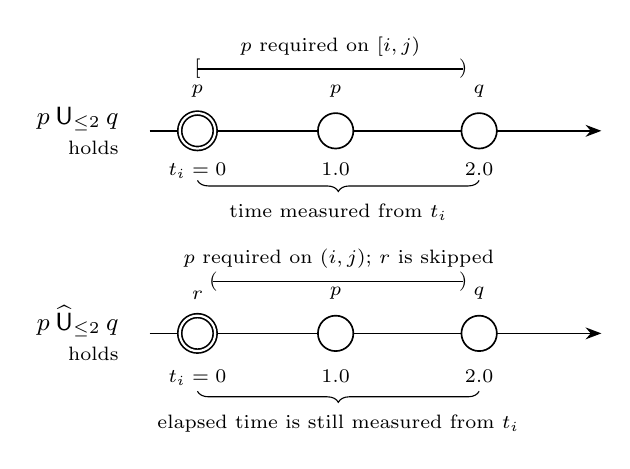
\begin{tikzpicture}[x=1.35cm,y=1.05cm,
  ival/.style={line width=0.5pt},
  ivallab/.style={font=\scriptsize,above=1pt}]
  % Ordinary Until
  \node[anchor=east,font=\small,align=right] at (-0.20,1.30) {$p\Until_{\le 2}q$\\{\scriptsize holds}};
  \draw[fmtimeline] (0,1.30) -- (4.25,1.30);
  \node[fmreference] (u0) at (0.45,1.30) {};
  \node[fmevent] (u1) at (1.75,1.30) {};
  \node[fmevent] (u2) at (3.10,1.30) {};
  \node[above=2pt of u0,font=\scriptsize] {$p$};
  \node[above=2pt of u1,font=\scriptsize] {$p$};
  \node[above=2pt of u2,font=\scriptsize] {$q$};
  \node[below=1.5pt of u0,font=\scriptsize] {$t_i=0$};
  \node[below=1.5pt of u1,font=\scriptsize] {$1.0$};
  \node[below=1.5pt of u2,font=\scriptsize] {$2.0$};
  \draw[ival] (0.45,2.05) -- (2.95,2.05);
  \node[font=\scriptsize] at (0.45,2.05) {$[$};
  \node[font=\scriptsize] at (2.95,2.05) {$)$};
  \node[ivallab] at (1.70,2.05) {$p$ required on $[i,j)$};
  \draw[fmbracebottom] (0.45,0.70) -- node[below=5pt,font=\scriptsize] {time measured from $t_i$} (3.10,0.70);

  % Hatted Until
  \node[anchor=east,font=\small,align=right] at (-0.20,-1.15) {$p\hUntil_{\le 2}q$\\{\scriptsize holds}};
  \draw[fmtimeline] (0,-1.15) -- (4.25,-1.15);
  \node[fmreference] (h0) at (0.45,-1.15) {};
  \node[fmevent] (h1) at (1.75,-1.15) {};
  \node[fmevent] (h2) at (3.10,-1.15) {};
  \node[above=2pt of h0,font=\scriptsize] {$r$};
  \node[above=2pt of h1,font=\scriptsize] {$p$};
  \node[above=2pt of h2,font=\scriptsize] {$q$};
  \node[below=3pt of h0,font=\scriptsize] {$t_i=0$};
  \node[below=3pt of h1,font=\scriptsize] {$1.0$};
  \node[below=3pt of h2,font=\scriptsize] {$2.0$};
  \draw[ival] (0.60,-0.52) -- (2.95,-0.52);
  \node[font=\scriptsize] at (0.60,-0.52) {$($};
  \node[font=\scriptsize] at (2.95,-0.52) {$)$};
  \node[ivallab] at (1.78,-0.52) {$p$ required on $(i,j)$; $r$ is skipped};
  \draw[fmbracebottom] (0.45,-1.85) -- node[below=5pt,font=\scriptsize] {elapsed time is still measured from $t_i$} (3.10,-1.85);
\end{tikzpicture}

\caption{Ordinary and hatted Until. The double circle is the timing reference.
The hatted operator skips the current event logically but measures from its
timestamp.}
\label{fig:hatted-until}
\end{figure}

Figure~\ref{fig:hatted-until} contrasts the two readings. The distinction is
useful for sporadicity: if consecutive occurrences of
$e$ must be separated by at least $\theta$, one may write
$\Box(e\Rightarrow\widehat{\Box}_{<\theta}\neg e)$. The hatted form retains
the triggering event as the time origin; ordinary bounded temporal
operators do not express this particular reference shift directly.
Related pointwise MTL constructions and the CASAAL translation are discussed
in prior work~\cite{ouaknine_worrell_lics05,bouyer_chevalier_markey_fsttcs05,li_spin7,casaal_tool}.

\subsection{Timed B\"uchi Automata}
\label{sec:tba}
The verified target is an event-guarded TBA
$\mathcal A=(L,\ell_0,X,E,\mathit{Acc})$. Here $L$ is a finite set of
locations, $\ell_0$ the initial location, $X$ a finite set of clocks,
$E\subseteq L\times\mathsf{Lab}\times\mathsf{Guard}\times 2^X\times L$
is the set of action-labeled transitions with guards and reset sets, and
$\mathit{Acc}\subseteq L$ the B\"uchi set. A run is a sequence
$(\ell_i,v_i)_{i\ge0}$ starting at $\ell_0$; it follows one transition per
event and visits $\mathit{Acc}$ infinitely often. If the selected edge at
event $i$ is $(\ell_i,\alpha_i,g_i,Z_i,\ell_{i+1})$, then the event action
must satisfy $\alpha_i$ and the valuation $v_i$ must satisfy every guard in
$g_i$. There are no location invariants in this model: timing constraints
are checked at the events of the timed word. This is the TBA record
represented in Rocq.

Let $v_i$ be the clock valuation tested at event $i$ and
$\Delta_i=t_{i+1}-t_i$. A transition at event $i$ tests $v_i$ before its
reset decision; the next valuation is
\[
v_{i+1}(x)=
\begin{cases}
\Delta_i,&x\in Z_i,\\
v_i(x)+\Delta_i,&\text{otherwise.}
\end{cases}
\]
The initial nonnegative valuation $v_0$ is existentially quantified, as in
the Rocq clock-consistent-extension semantics; standard zero initialization
is not assumed.

\section{Clocked-LTL Translation}
\label{sec:translation}
\subsection{Shared clock identities}
The translation is structural. It maps Boolean and untimed temporal
operators to their LTL counterparts and maps each primitive timed subformula to an LTL
formula over an extended alphabet. For each action $a$, the extended
alphabet contains distinct action atoms $\mathsf{LAct}(a)$ and
$\mathsf{LNAct}(a)$, as well as clock-related atoms: clock comparisons
$x\sim d$, a reset atom
$\Reset(x)$, and a preservation atom $\Unch(x)$. Under timed-word
interpretation, the action atoms mean that the current action is $a$ or is
different from $a$, respectively. The reset
and preservation atoms describe the clock update at the current event. Clock
values are read before the event's reset, matching the guard semantics of a
timed automaton.

For a formula $f$, let $\Clock(f)$ be its finite set of distinct primitive
hatted timed subformulas. The clock associated with $F\in\Clock(f)$ is
$x=F$ itself. Clock identity uses structural equality on the Rocq MTL syntax
tree. The main result proves that this clock
also serves all dynamic activations of its subformula.
The clock count is therefore bounded by the number of distinct primitive
timed subformulas, which is at most the number of timed occurrences in $f$.
If structural subformulas are represented as shared nodes, the translation
can share their LTL encodings as well; this does not remove the usual
worst-case growth of an LTL-to-B\"uchi construction.

This clock-sharing policy is distinct from automaton-state minimization. The
reset trace is chosen for each formula identity as a whole. In particular,
the proof cannot justify the clock bound
by assigning a fresh clock to each activation and subsequently identifying
those clocks: it establishes directly that a single trace of reset decisions
for the formula is sufficient.

\subsection{Eight primitive clauses}
\label{sec:mtlbuchi}
Let $F$ be a primitive hatted formula at path $\pi$, with operands $p,q$.
Write $x=\mathsf{clock\_of}(F)$, $P=\T_{\pi0}(p)$,
$Q=\T_{\pi1}(q)$, and define
$\alpha\WeakUntil\beta=(\alpha\Until\beta)\lor\Always\alpha$.
For upper comparisons $\precsim\in\{\le,<\}$ and lower comparisons
$\succsim\in\{\ge,>\}$, complements are
$\le^{\mathrm c}=>$, $<^{\mathrm c}=\ge$, $\ge^{\mathrm c}=<$, and
$>^{\mathrm c}=\le$. The four clause shapes give all eight primitive cases:
\begin{align}
\T_\pi(p\hUntil_{\precsim d}q)
 &=\Next\bigl(((x\precsim d)\land\Unch(x)\land P)\nonumber\\
 &\hspace{23mm}\Until((x\precsim d)\land Q)\bigr),\label{eq:t-hule}\\
\T_\pi(p\hUntil_{\succsim d}q)
 &=\Reset(x)\land\Next\bigl((P\Until((x\succsim d)\land(P\Until Q)))\nonumber\\
 &\hspace{23mm}\lor(\Always P\land\Always\Eventually Q)\bigr),\label{eq:t-huge}\\
\T_\pi(p\hRelease_{\precsim d}q)
 &=\Reset(x)\land\Next\bigl(Q\nonumber\\
 &\hspace{23mm}\WeakUntil((x\mathrel{\precsim^{\mathrm c}}d)\lor(P\land Q))\bigr),\label{eq:t-hrle}\\
\T_\pi(p\hRelease_{\succsim d}q)
 &=\Next\bigl(((x\mathrel{\succsim^{\mathrm c}}d)\land\Unch(x))\nonumber\\
 &\hspace{23mm}\WeakUntil((P\Release Q)\nonumber\\
 &\hspace{23mm}\lor((x\mathrel{\succsim^{\mathrm c}}d)\land P))\bigr).
 \label{eq:t-hrge}
\end{align}
The outer $\Next$ implements the hatted shift; $\Reset(x)$ and $\Unch(x)$
encode the restart and preservation choices. Until uses strong Until for a
bounded witness and weak Until for the Release window. Lower-bounded Until
also has a fairness branch for an obligation whose threshold is delayed
indefinitely. Every clock atom occurs positively, which is the property used
by relaxation in Section~\ref{sec:reset-completion}. The eight local proof
arguments establish the precise behavior in
Section~\ref{subsec:primitive-soundness}.

\subsection{Shared clocks under overlapping activations}
\label{subsec:overlap-motivation}
Hatted operators preserve the triggering timestamp while moving logical
evaluation to the next event. For example,
$\Box(e\Rightarrow\widehat{\Box}_{<\theta}\neg e)$ measures an exclusion
window from the triggering event. The leading next in an ordinary operator
would shift that reference, while omitting it also constrains the triggering
event. Fig.~\ref{fig:hat-reference} contrasts these readings.
\begin{figure*}[t]
\centering
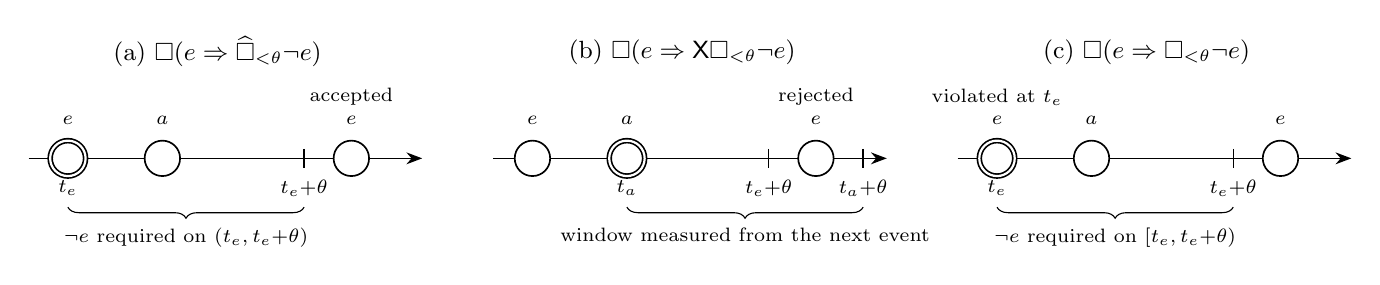
\begin{tikzpicture}[x=1cm,y=1cm,
  tick/.style={line width=0.5pt},
  ticklab/.style={font=\scriptsize,below=1pt},
  verdict/.style={fmnote}]
  % (a) Hatted operator: the intended reading
  \begin{scope}[xshift=0cm]
    \node[font=\small] at (2.4,1.35) {(a) $\Box(e\Rightarrow\widehat{\Box}_{<\theta}\neg e)$};
    \draw[fmtimeline] (0,0) -- (5.0,0);
    \node[fmreference] (a0) at (0.5,0) {};
    \node[fmevent] (a1) at (1.7,0) {};
    \node[fmevent] (a2) at (4.1,0) {};
    \node[above=2pt of a0,font=\scriptsize] {$e$};
    \node[above=2pt of a1,font=\scriptsize] {$a$};
    \node[above=2pt of a2,font=\scriptsize] {$e$};
    \node[verdict] at (4.1,0.78) {accepted};
    \draw[tick] (3.5,0.12) -- (3.5,-0.12) node[ticklab] {$t_e{+}\theta$};
    \node[ticklab] at (0.5,-0.12) {$t_e$};
    \draw[fmbracebottom] (0.5,-0.62) -- node[below=4pt,fmnote] {$\neg e$ required on $(t_e,t_e{+}\theta)$} (3.5,-0.62);
  \end{scope}

  % (b) Replacing the hat by a leading Next
  \begin{scope}[xshift=5.9cm]
    \node[font=\small] at (2.4,1.35) {(b) $\Box(e\Rightarrow\Next\Box_{<\theta}\neg e)$};
    \draw[fmtimeline] (0,0) -- (5.0,0);
    \node[fmevent] (b0) at (0.5,0) {};
    \node[fmreference] (b1) at (1.7,0) {};
    \node[fmevent] (b2) at (4.1,0) {};
    \node[above=2pt of b0,font=\scriptsize] {$e$};
    \node[above=2pt of b1,font=\scriptsize] {$a$};
    \node[above=2pt of b2,font=\scriptsize] {$e$};
    \node[verdict] at (4.1,0.78) {rejected};
    \draw[tick] (3.5,0.12) -- (3.5,-0.12) node[ticklab] {$t_e{+}\theta$};
    \draw[tick] (4.7,0.12) -- (4.7,-0.12) node[ticklab] {$t_a{+}\theta$};
    \node[ticklab] at (1.7,-0.12) {$t_a$};
    \draw[fmbracebottom] (1.7,-0.62) -- node[below=4pt,fmnote] {window measured from the next event} (4.7,-0.62);
  \end{scope}

  % (c) Dropping the Next
  \begin{scope}[xshift=11.8cm]
    \node[font=\small] at (2.4,1.35) {(c) $\Box(e\Rightarrow\Box_{<\theta}\neg e)$};
    \draw[fmtimeline] (0,0) -- (5.0,0);
    \node[fmreference] (c0) at (0.5,0) {};
    \node[fmevent] (c1) at (1.7,0) {};
    \node[fmevent] (c2) at (4.1,0) {};
    \node[above=2pt of c0,font=\scriptsize] {$e$};
    \node[above=2pt of c1,font=\scriptsize] {$a$};
    \node[above=2pt of c2,font=\scriptsize] {$e$};
    \node[verdict] at (0.5,0.78) {violated at $t_e$};
    \draw[tick] (3.5,0.12) -- (3.5,-0.12) node[ticklab] {$t_e{+}\theta$};
    \node[ticklab] at (0.5,-0.12) {$t_e$};
    \draw[fmbracebottom] (0.5,-0.62) -- node[below=4pt,fmnote] {$\neg e$ required on $[t_e,t_e{+}\theta)$} (3.5,-0.62);
  \end{scope}
\end{tikzpicture}

\caption{The hatted sporadicity property and two ordinary-operator
substitutions. A leading next shifts the timing reference to the following
event; omitting it includes the triggering event in the window.}
\label{fig:hat-reference}
\end{figure*}

The proof assigns one clock to each structurally distinct primitive timed
formula, even when that formula is activated repeatedly. The finite prefix in
Table~\ref{tab:overlap-example} illustrates why completeness must account for
all pending obligations: resetting a single clock at the later request can
make an expired earlier deadline appear to be met.
\begin{table}[t]
\centering
\caption{A finite prefix illustrating overlapping response obligations.
The deadline is five time units; the acknowledgment at time six is late for
the request at time zero even though it is age two from the later request.}
\label{tab:overlap-example}
\begin{tabular}{@{}clccc@{}}
\toprule
Event $i$ & Action & Time $t_i$ & Oldest age & Reset age\\
\midrule
0 & $\mathit{req}$ & 0 & 0 & 0\\
1 & $\mathit{req}$ & 4 & 4 & 4\\
2 & $\mathit{ack}$ & 6 & 6 & 2\\
\bottomrule
\end{tabular}
\end{table}
The semantic proof below constructs one trace per
formula-keyed clock and establishes the residual invariants needed when
several activations are pending at once.

\section{From Clocked LTL to a TBA}
\label{sec:tba-construction}
\subsection{LTL-to-B\"uchi contract}
The backend treats the clock-related atoms as independent propositions and
receives the negated action atom $\mathsf{LNAct}(a)$ as the negation of the
action atom $\mathsf{LAct}(a)$. It returns a propositional B\"uchi automaton
(PBA) whose language is exactly that of the clocked-LTL formula. The theorem is
stated for any such backend, deterministic or not. A propositional word is
\emph{action-consistent} when, at every position, $\mathsf{LNAct}(a)$ holds
exactly when $\mathsf{LAct}(a)$ does not.
\begin{assumption}[Backend correctness]
\label{ass:backend}
For each formula $F$ and each action-consistent propositional word $s$ over
its atoms, $\mathsf{PBA\_accepts}(A,s)$ iff $s,0\models F$, where $A$ is the
backend automaton for $F$.
\end{assumption}
This contract ranges over all action-consistent propositional words,
including assignments of the clock-related atoms that do not correspond to any
clock-consistent timed word. That scope is used by relaxation. 

\subsection{Relaxation and reset completion}
\label{sec:reset-completion}
The propositional backend regards every clock-related atom as independent.
Its correctness contract therefore applies to all action-consistent Boolean
words, including assignments of the clock-related atoms that cannot arise from
any clock-consistent timed trace. Every
clock-related atom in the translation occurs positively. Relaxation acts on
each backend transition cube (conjunction of atomic constraints) by removing negative literals over clock
comparisons and reset/preservation markers, removing irrelevant
clock-related literals, and discarding contradictory cubes. Action literals
and positive relevant clock literals are retained. This weakens the cubes
without asking the backend to understand clocks.

Reset completion converts each relaxed cube to a timed transition. Clocks of
upper-bounded hatted Until and lower-bounded hatted Release are preservation
clocks (their clauses use $\Unch$); clocks of lower-bounded hatted Until and
upper-bounded hatted Release are restart clocks (their clauses use $\Reset$). A
preservation clock is reset unless the cube contains $\Unch(x)$; a restart
clock is reset exactly when the cube contains $\Reset(x)$. The markers are
then removed, clock comparisons become guards, and action literals become
labels. The two clock classes move in opposite directions, so the proof
treats them separately.

\begin{lemma}[Reset completion]
\label{lem:reset-completion}
Let an accepting run of the relaxed backend be accompanied by a
clock-consistent extension $\rho$ of its timed word. Reset completion
defines a clock-consistent extension $\rho'$ with the same timed word and
the same initial clock valuation. The same state sequence is an accepting
run of the completed TBA on $\rho'$.
\end{lemma}
\begin{proof}
Fix a selected backend cube at position $i$. For a preservation clock $x$,
if the cube contains $\Unch(x)$ then both traces preserve $x$. Otherwise the
completed TBA resets $x$, while $\rho$ may either reset it or preserve it.
Thus the completed reset set contains the original reset decision for $x$.
Induction on positions using the clock recurrence gives
$\CVal_{\rho'}(i,x)\le\CVal_\rho(i,x)$. These clocks occur only in upper
tests ($x\precsim d$), which remain true when the value decreases.

For a restart clock $x$, completion resets it exactly when the cube contains
$\Reset(x)$. A true reset marker requires that $\rho$ resets $x$; without the
marker completion preserves it, whether or not $\rho$ resets it. The
completed reset set is therefore contained in the original one, and the same
induction gives $\CVal_{\rho'}(i,x)\ge\CVal_\rho(i,x)$. These clocks occur
only in lower tests ($x\succsim d$, or their equivalent window-ending
comparisons), which remain true when the value increases. The clock recurrence
holds by the construction of $\rho'$. State transitions, event labels,
guards that remain true, and the Büchi accepting set are unchanged, so the
run remains accepting. Rocq proves this result as
\Rocqid{complete_complete}.
\end{proof}

\subsection{Worked example: bounded eventuality with an exclusion window}
Let
\[
  f=(\Eventually_{\le5}p)\land(\Always_{<2}\neg p).
\]
It requires $p$ to be false at the origin and until age two, then true by age
five. Fig.~\ref{fig:translation-reference-tba} shows a hand-simplified
equivalent one-clock TBA, not the syntax-directed output, which assigns
separate clocks to the two distinct timed subformulas. The steps below show
the clocked-LTL translation and timed reinterpretation. This is a construction
illustration: the saved Spot graph and its two-clock TBA transcription are not
covered by the proved Rocq backend contract. The concrete instance
checked in Rocq is the alarm-response example in
Section~\ref{sec:alarm-example}.

\begin{figure}[t]
\centering
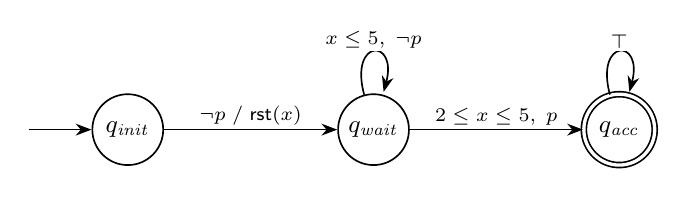
\begin{tikzpicture}[node distance=22mm]
  \node[fmstate] (q0) {$q_{\mathit{init}}$};
  \node[fmstate,right=of q0] (q1) {$q_{\mathit{wait}}$};
  \node[fmaccept,right=of q1] (q2) {$q_{\mathit{acc}}$};
  \draw[fmedge] ([xshift=-8mm]q0.west) -- (q0.west);
  \draw[fmedge] (q0) -- node[fmlabel,above] {$\neg p\;/\;\mathsf{rst}(x)$} (q1);
  \draw[fmedge] (q1) edge[loop above] node[fmlabel] {$x\le5,\;\neg p$} (q1);
  \draw[fmedge] (q1) -- node[fmlabel,above] {$2\le x\le5,\;p$} (q2);
  \draw[fmedge] (q2) edge[loop above] node[fmlabel] {$\top$} (q2);
\end{tikzpicture}

\caption{Hand-simplified equivalent event-guarded TBA for $f$. The initial
transition requires $\neg p$ and resets $x$; in the waiting location,
$x\le5$, and acceptance also requires $x\ge2$. Thus $p$ first holds at age
in $[2,5]$.}
\label{fig:translation-reference-tba}
\end{figure}

\begin{enumerate}[label=Step~\arabic*:,leftmargin=*]
\item The formula is in negation normal form. Expanding the derived operators
and applying the timed-operator identities gives
\[
\begin{aligned}
f
 &= (\top\Until_{\le5}p)\land(\bot\Release_{<2}\neg p)\\
 &= \bigl(p\lor(\top\land\top\hUntil_{\le5}p)\bigr)\\
 &\qquad\land\bigl(\neg p\land(\bot\lor\bot\hRelease_{<2}\neg p)\bigr).
\end{aligned}
\]
These current-position cases follow Eqs.~\eqref{eq:derive-ule} and
\eqref{eq:derive-rle}.

\item The two distinct primitive timed subformulas receive clocks $x$ and
$y$, respectively. Their clocked-LTL translation is
\begin{align*}
\Phi_U={}&p\lor\bigl(\top\land\Next\Bigl(
  ((x\le5)\land\Unch(x)\land\top)\Until\\[-1mm]
&\qquad((x\le5)\land p)\Bigr)\bigr),\\[-1mm]
\Phi_R={}&\neg p\land\bigl(\bot\lor(\Reset(y)\land\\[-1mm]
&\qquad\Next(\neg p\WeakUntil((y\ge2)\lor(\bot\land\neg p))))\bigr),\\[-1mm]
\T(f)={}&\Phi_U\land\Phi_R.
\end{align*}
The Until clause preserves $x$; the Release test $y\ge2$ complements the source
bound $<2$, allowing $p$ from age two.

\item The saved Spot 2.16 graph for $\T(f)$ is redrawn on the left of
Fig.~\ref{fig:translation-steps45} (top). The clock guards $x\le5$ and
$y\ge2$, the markers $\mathsf{unch}(x)$ and $\mathsf{rst}(y)$, and the action
atom $p$ are propositions to the backend, and the negated action atom
$\neg p=\mathsf{LNAct}(p)$ reaches Spot as the negation of the atom $p$
(the default of the tool; Section~\ref{sec:tba-construction}). No cube of
the graph therefore contains both $p$ and $\neg p$, and every edge is
realizable by a timed event. The graph has four
states and seven transitions, the size reported for F11 in
Table~\ref{tab:compiled}.

\item Relaxation removes negative literals over extended clock atoms, here
$\neg(y\ge2)$. Reset completion resets the preservation clock $x$ unless
$\mathsf{unch}(x)$ is present; the restart clock $y$ is reset exactly when
$\mathsf{rst}(y)$ is present. The bottom of
Fig.~\ref{fig:translation-steps45} shows the same state graph after these
operations: each edge carries the event, the clock guard, and the resets. The
event is an action ($p$ or $\neg p$), and $\top$ stands for any event.
\end{enumerate}

\begin{figure*}[!t]
\centering
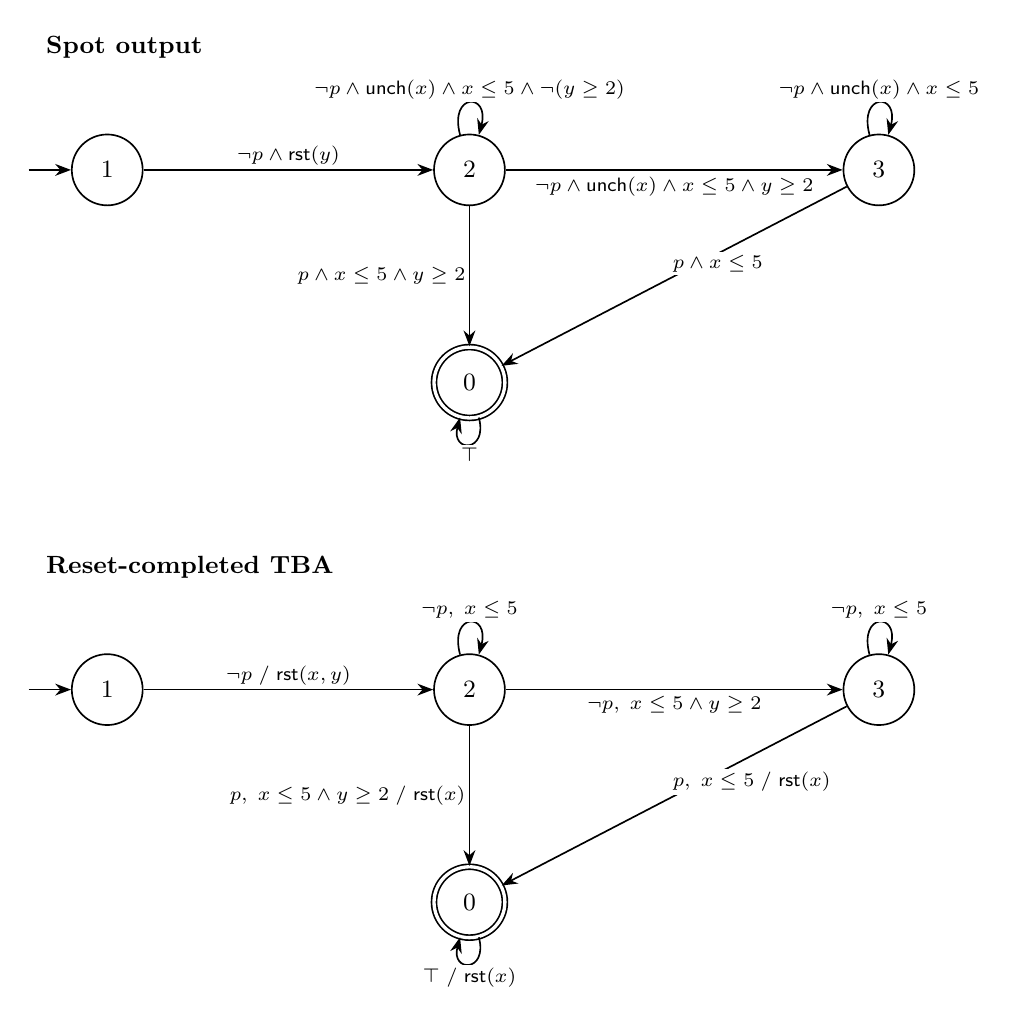
\begin{tikzpicture}[x=1cm,y=1cm]
% Left: the saved Spot graph for T(f) (negated event atom printed as !"p").
% Right of the arrows: guards and resets of the reset-completed TBA.
\begin{scope}[xshift=0cm]
  \node[fmnote,font=\small\bfseries,anchor=west] at (-0.9,1.55) {Spot output};
  \node[fmstate] (a0) at (0.0,0.0) {$1$};
  \node[fmstate] (a1) at (4.6,0.0) {$2$};
  \node[fmstate] (a3) at (9.8,0.0) {$3$};
  \node[fmaccept] (a2) at (4.6,-2.7) {$0$};
  \draw[fmedge] (-1.0,0.0) -- (a0);
  \draw[fmedge] (a0) -- node[fmlabel,above] {$\neg p\land\mathsf{rst}(y)$} (a1);
  \draw[fmedge] (a1) edge[loop above,looseness=6]
    node[fmlabel] {$\neg p\land\mathsf{unch}(x)\land x\le5\land\neg(y\ge2)$} (a1);
  \draw[fmedge] (a1) -- node[fmlabel,below,yshift=-1pt] {$\neg p\land\mathsf{unch}(x)\land x\le5\land y\ge2$} (a3);
  \draw[fmedge] (a1) -- node[fmlabel,left] {$p\land x\le5\land y\ge2$} (a2);
  \draw[fmedge] (a3) edge[loop above,looseness=6]
    node[fmlabel] {$\neg p\land\mathsf{unch}(x)\land x\le5$} (a3);
  \draw[fmedge] (a3) -- node[fmlabel,above right,xshift=-2pt] {$p\land x\le5$} (a2);
  \draw[fmedge] (a2) edge[loop below,looseness=5] node[fmlabel] {$\top$} (a2);
\end{scope}

\begin{scope}[yshift=-6.6cm]
  \node[fmnote,font=\small\bfseries,anchor=west] at (-0.9,1.55) {Reset-completed TBA};
  \node[fmstate] (b0) at (0.0,0.0) {$1$};
  \node[fmstate] (b1) at (4.6,0.0) {$2$};
  \node[fmstate] (b3) at (9.8,0.0) {$3$};
  \node[fmaccept] (b2) at (4.6,-2.7) {$0$};
  \draw[fmedge] (-1.0,0.0) -- (b0);
  \draw[fmedge] (b0) -- node[fmlabel,above] {$\neg p\;/\;\mathsf{rst}(x,y)$} (b1);
  \draw[fmedge] (b1) edge[loop above,looseness=6]
    node[fmlabel] {$\neg p,\;x\le5$} (b1);
  \draw[fmedge] (b1) -- node[fmlabel,below,yshift=-1pt] {$\neg p,\;x\le5\land y\ge2$} (b3);
  \draw[fmedge] (b1) -- node[fmlabel,left] {$p,\;x\le5\land y\ge2\;/\;\mathsf{rst}(x)$} (b2);
  \draw[fmedge] (b3) edge[loop above,looseness=6]
    node[fmlabel] {$\neg p,\;x\le5$} (b3);
  \draw[fmedge] (b3) -- node[fmlabel,above right,xshift=-2pt] {$p,\;x\le5\;/\;\mathsf{rst}(x)$} (b2);
  \draw[fmedge] (b2) edge[loop below,looseness=5] node[fmlabel] {$\top\;/\;\mathsf{rst}(x)$} (b2);
\end{scope}
\end{tikzpicture}

\caption{The saved Spot 2.16 graph for $\T(f)$ (top, redrawn; the labels are
propositional cubes over the action atom $p$, the clock guards, and the markers
$\mathsf{unch}(x)$ and $\mathsf{rst}(y)$) and the reset-completed TBA obtained
from it by hand (bottom; same state numbers). A TBA edge is labeled
by the event, the clock guard, and, after a slash, the clocks reset; $\top$ is
any event, and an edge without a slash resets no clock. This graph-to-TBA
illustration is not the formally verified alarm-response backend instance.}
\label{fig:translation-steps45}
\end{figure*}


\section{Mechanized Correctness}
\label{sec:correctness}
\label{sec:encoding-correctness}
For a formula $f$, an extended word $\rho$ augments the timed word with a
nonnegative value $\CVal_\rho(i,x)$ and a reset decision
$\CReset_\rho(i,x)$ for every formula-keyed clock $x\in\Clock(f)$ at each
position $i$. It is clock-consistent when, with
$\Delta_i=t_{i+1}-t_i$,
\begin{equation}
\CVal_\rho(i+1,x)=
\begin{cases}
\Delta_i,&\CReset_\rho(i,x),\\
\CVal_\rho(i,x)+\Delta_i,&\text{otherwise.}
\end{cases}
\label{eq:clock-update}
\end{equation}
The value at $i$ is tested before the reset decision at $i$. The relation
$\mathsf{same\_base}(\rho,w)$ means that the projection of $\rho$ onto actions
and timestamps gives $w$.

\subsection{Soundness for arbitrary reset traces}
\label{subsec:primitive-soundness}
The soundness direction does not select or assume any particular reset
policy; in particular, it does not use the canonical policy that
Section~\ref{subsec:canonical-policy} defines for completeness. For
each primitive formula $F$ at path $\pi$, the corresponding Rocq lemma
\texttt{sound\_*} turns $\rho,i\satL\T_\pi(F)$ into
$\ewbase(\rho),i\satM F$, assuming clock consistency and
induction hypotheses for its operands. 
Clock consistency gives two useful bounds. If a clock is preserved on
$[i,j)$, then
\[
\CVal_\rho(j,x)=\CVal_\rho(i,x)+\elapsed_w(i,j).
\]
Since clock values are nonnegative, preservation implies
$\CVal_\rho(j,x)\ge\elapsed_w(i,j)$. If it is reset at $i$, then for every
$j\ge i+1$,
\[
\CVal_\rho(j,x)\le\elapsed_w(i,j),
\]
with equality when it is not reset again before $j$. The upper-guard
implication follows from the first inequality; the lower-guard implication
follows from the second. Both follow by induction from
Eq.~\eqref{eq:clock-update} and nonnegative delays.

\runinhead{Upper-bounded hatted Until.}
The outer $\Next$ moves to the first strictly future event. The strong Until
then supplies a witness $j>i$ satisfying $Q$, with $P$ at every intermediate
event and $\Unch(x)$ throughout that prefix. Regardless of whether the clock
was reset at $i$, its value at $i+1$ is at least $\Delta_i$.
Preservation after $i+1$ therefore gives
\[
\CVal_\rho(j,x)\ge
\Delta_i+\elapsed_w(i+1,j)=\elapsed_w(i,j).
\]
The endpoint guard $x\le d$ implies $\elapsed_w(i,j)\le d$; the guard $x<d$
implies $\elapsed_w(i,j)<d$. Induction on $P,Q$ yields the hatted Until
witness and prefix in both cases. The strong Until is essential: an infinite
continuation with no $Q$ endpoint is not a bounded Until witness.

\runinhead{Lower-bounded hatted Until.}
Here the translation requires $\Reset(x)$ at $i$. The finite branch (the first disjunct of
Eq.~\eqref{eq:t-huge}) waits for a position with $x\succsim d$ and then supplies an
ordinary $P\Until Q$ witness. Since subsequent resets can only make a clock
younger, $\CVal_\rho(j,x)\le\elapsed_w(i,j)$; thus the threshold guard proves
the required lower-bound comparison. The nested Until supplies $P$ up to the
$Q$ witness. The other branch is
$\Always P\land\Always\Eventually Q$. It gives an unbroken $P$ prefix and
unboundedly many $Q$ positions; divergence of timestamps lets us choose a
$Q$ witness beyond any finite lower bound. For the strict case, choose a
recurring $Q$ at distance at least $d$ from $i+1$. Since
$t_{i+1}>t_i$, that same event is strictly more than $d$ after $i$. This is
the additional argument in \Rocqid{sound_UhatGt}; it preserves the strict
boundary without changing the constant.

\runinhead{Upper-bounded hatted Release.}
The translation resets the clock at $i$ and uses weak Until with $Q$ as its
left condition. Consequently, $Q$ holds at each future event until either
$P\land Q$ discharges the Release obligation or the complementary clock test
marks the end of the upper window. For a non-strict upper bound, the window
ends at $x>d$; for a strict upper bound, it ends at $x\ge d$. If the clock
has been reset again, its value is no larger than the elapsed time from $i$,
so either endpoint guard can hold only after the corresponding physical-time
window has ended. If weak Until ends at $P\land Q$, $P$ at that earlier event
discharges later Release obligations. This proves both comparisons with their
exact strict boundary.

\runinhead{Lower-bounded hatted Release.}
Before the threshold, the left side of weak Until requires both the
pre-threshold comparison and $\Unch(x)$. Thus an arbitrary reset trace
cannot move the clock backwards while the pre-threshold condition remains
active. Once the comparison becomes false, the translation requires ordinary
$P\Release Q$ from that event, unless the right-side alternative has already
terminated the obligation at a position satisfying $P$ while still below the
threshold. An older initial clock value can make the translation enter the
ordinary Release branch earlier than the MTL interval does; this only imposes
a stronger condition. 

The standard LTL semantics used here are formalized in Rocq as
\Rocqid{LG_semantics}, \Rocqid{LGF_semantics},
\Rocqid{LW_semantics}, and \Rocqid{LF_semantics}. Time divergence is used
only for the fairness witness in lower-bounded Until; no assumption on the
reset policy beyond clock consistency is used in any soundness family.

\subsection{Canonical reset policy and residual obligations}
\label{subsec:canonical-policy}
Completeness must choose one clock trace for each primitive formula, even
when activations overlap. The canonical policy preserves a reference only
while its residual obligation is still useful. Recall that
$\elapsed_w(i,j)=t_j-t_i$. For upper-bounded Until define
\begin{align}
\mathsf{URes}_{\precsim}(i,v,d,p,q)\iff{}
&\exists j\ge i.\;v+\elapsed_w(i,j)\precsim d\nonumber\\[-1mm]
&\land w,j\satM q\nonumber\\[-1mm]
&\land\forall k\in[i,j).\,w,k\satM p\label{eq:ures-le}
\end{align}
The residual says that a $q$ endpoint is still reachable with the current
clock age and the required $p$ prefix. For lower-bounded Release define
\begin{align}
\mathsf{RRes}_{\succsim}(i,v,d,p,q)\iff{}
&\forall j\ge i.\;v+\elapsed_w(i,j)\succsim d\Rightarrow\nonumber\\[-1mm]
&\Bigl(w,j\satM q~\lor\nonumber\\[-1mm]
&\exists k\in[i,j).\,w,k\satM p\Bigr)\label{eq:rres-ge}
\end{align}
The residual $\mathsf{RRes}$ is universal: every position already beyond the
threshold must have $q$ or an earlier $p$ that discharges the obligation;
$\mathsf{URes}$ is its existential counterpart (a reachable $q$ endpoint).
Instantiating $\precsim$ as $\le$ or $<$, and $\succsim$ as $\ge$ or $>$,
gives the non-strict and strict variants.

For a clock $x=F$, let $v=\CVal_{\rho^\star}(i,x)$; Table~\ref{tab:canonical-policy} gives the
policy.
\begin{table}[t]
\centering
\caption{Canonical reset decision at position $i$, with $\precsim$ ranging over
$\{\le,<\}$ and $\succsim$ over $\{\ge,>\}$. A preservation row gives
the condition under which the clock is not reset; otherwise it is reset.}
\label{tab:canonical-policy}
\begin{tabular}{@{}p{0.35\columnwidth}p{0.59\columnwidth}@{}}
\toprule
Primitive formula $F$ & Decision at $i$\\
\midrule
$p\hUntil_{\precsim d}q$ &
Preserve iff $v\precsim d$, $\mathsf{URes}_{\precsim}(i,v,d,p,q)$, and
$w,i\not\satM q$.\\
$p\hUntil_{\succsim d}q$, $p\hRelease_{\precsim d}q$ &
Reset iff $w,i\satM F$.\\
$p\hRelease_{\succsim d}q$ &
Preserve iff $v\not\succsim d$, $\mathsf{RRes}_{\succsim}(i,v,d,p,q)$, and
$w,i\not\satM p$.\\
\bottomrule
\end{tabular}
\end{table}
The resulting values begin at $u_0=0$ and evolve by
\[
u_{i+1}=
\begin{cases}
\Delta_i,&\text{if the policy resets at }i,\\
u_i+\Delta_i,&\text{otherwise.}
\end{cases}
\]
This is a word-dependent completeness witness, not a reset algorithm in an
executable translator. Its decisions are keyed by the primitive formula
itself, not by an occurrence path.

\subsection{Completeness for one canonical trace}
\label{subsec:primitive-completeness}
For every formula satisfied by $w$, completeness constructs one clock-consistent
extension $\rho^\star$ that serves all activations of every shared clock.
The four operator families use different invariants:

\runinhead{Upper-bounded hatted Until.}
Choose the first position $j>i$ at which $q$ holds with $p$ on $[i,j)$, while
the activation remains pending. The
key invariant along the translated strong-Until prefix is
\begin{equation}
\CVal_{\rho^\star}(n,x)+\elapsed_w(n,j)\le d
\quad(i<n\le j).
\label{eq:canonical-until-invariant}
\end{equation}
For $<d$, replace $\le d$ by $<d$. The invariant need not hold at $i$:
the translation begins with $\Next$, so the first clock test is at $i+1$.
If the policy resets at $i$, then $u_{i+1}=\Delta_i$ and
$u_{i+1}+\elapsed_w(i+1,j)=\elapsed_w(i,j)$, which is within the bound for
the chosen witness. If it preserves at $i$, the residual supplies a still
reachable $q$ endpoint and $p$ prefix; because the current $q$ has not
discharged that residual, its witness is strictly after $i$, and the same
identity advances the residual inequality to $i+1$. Because $j$ is the first such
position, $q$ fails at every intermediate position $n$ with $i<n<j$: otherwise
$n$ would be an earlier witness, since $p$ holds on $[i,n)\subseteq[i,j)$. The
invariant gives $\CVal_{\rho^\star}(n,x)+\elapsed_w(n,j)\le d$, so
$\mathsf{URes}_{\le}$ holds at $n$ with witness $j$. Hence the policy preserves
the reference at every intermediate position, which is what the conjunct
$\Unch(x)$ of the translation requires; the endpoint $j$ satisfies $q$ and the
clock comparison. A reference reset earlier has a larger age than any later
one, so if it still reaches the shared endpoint within $d$, the obligations of
the later activations are covered as well. This is the invariant proved
by \Rocqid{complete_UhatLe} and \Rocqid{complete_UhatLt}.

\runinhead{Lower-bounded hatted Until.}
Whenever the formula is true at an activation, the policy resets its clock.
Starting from $i+1$, a first position at which the canonical clock reaches
$d$ (or strictly exceeds $d$) and has a qualifying later $q$ witness gives
the finite branch (the first disjunct of Eq.~\eqref{eq:t-huge}): the clock guard supplies the lower-bound
test, and the nested $P\Until Q$ supplies the remaining witness. Before the
first such position, the proof maintains an active-witness invariant. At
each $n\ge i+1$ it supplies an activation $s<n$, a witness $m\ge n$ with
$t_m-t_s\ge d$ and $w,m\models q$, $p$ at every intermediate position, and
$\CVal_{\rho^\star}(n,x)=t_n-t_s$. Thus $p$ holds at $n$ and a $q$ witness
remains at or after every $n$. If a first qualifying position occurs, the
finite branch applies; if none occurs, the invariant yields
$\Always P\land\Always\Eventually Q$, the fairness branch (the second disjunct of Eq.~\eqref{eq:t-huge}).
Divergence converts recurring $q$ positions into a witness beyond the
lower bound. These are the arguments
formalized by \Rocqid{complete_UhatGe} and \Rocqid{complete_UhatGt}.

\runinhead{Upper-bounded hatted Release.}
At every activation where the hatted Release formula is true, the policy
resets the restart clock. The first future event must satisfy $q$, as
required by the hatted Release semantics. The universal condition then
continues as weak Until: $q$ holds until either $p\land q$ discharges all
later points or the clock passes the end of the bounded window. For a
$\le d$ window the stopping guard is $x>d$; for a $<d$ window it is
$x\ge d$. Resetting at a later true activation can extend the clock window,
but the later formula's truth supplies the corresponding future
$q$-or-discharge condition. Thus a single reset trace satisfies both the old
and new obligations. This proves \Rocqid{complete_RhatLe} and
\Rocqid{complete_RhatLt}.

\runinhead{Lower-bounded hatted Release.}
While $\mathsf{RRes}_{\ge}$ holds, $v<d$, and $p$ has not discharged the
obligation, the policy preserves the clock. Preservation advances both the
clock and the residual by
\[
(i,v)\longmapsto(i+1,v+\Delta_i),
\qquad
\elapsed_w(i,j)=\Delta_i+\elapsed_w(i+1,j).
\]
Substitution in Eq.~\eqref{eq:rres-ge} proves
$\mathsf{RRes}_{\ge}(i+1,v+\Delta_i,d,p,q)$. The instance $\succsim\,=\,>$
proves the same shift for $\mathsf{RRes}_{>}$ when $v\le d$. The residual ensures that
every event in the already-entered lower-bound region has $q$ or an earlier
$p$. If $p$ occurs while the clock is still below threshold, the right side
of weak Until terminates with that $p$; otherwise the clock reaches the
threshold and the residual supplies the ordinary Release continuation.
For $\ge d$, an event exactly at $d$ is already in the constrained region;
for $>d$, the prefix includes equality and only a strictly later event
starts the region. The corresponding proofs are
\Rocqid{complete_RhatGe}, \Rocqid{rge_residual_shift},
\Rocqid{complete_RhatGt}, and \Rocqid{rgt_residual_shift}.

\subsection{Occurrence-indexed structural induction}
\label{subsec:occurrence-induction}
The completeness proof must recurse through a syntax tree while preserving
the root formula's clock identities. Write
$\mathsf{node}(root,\pi)=f$ when the path lookup at $\pi$ in $root$
returns $f$ (the Rocq notation is
\texttt{node\_at root pi = Some f}). Let
$\rho^\star=\mathsf{canonical\_ext}(root,w)$. The strengthened theorem is:
\begin{theorem}[Canonical correctness at every syntactic occurrence]
\label{thm:canonical-all}
For every well-formed root formula, every path $\pi$ with
$\mathsf{node}(root,\pi)=f$, and every position $i$,
\[
w,i\satM f
\quad\Longleftrightarrow\quad
\rho^\star,i\satL\T_\pi(f).
\]
The same extension $\rho^\star$ is constructed once from $root$ and $w$ and
is used for all paths.
\end{theorem}
\begin{proof}
Proceed by structural induction on $f$. Boolean and untimed temporal cases
follow from their semantics and the induction hypotheses. For a binary
constructor, \Rocqid{node_at_left_binary} and
\Rocqid{node_at_right_binary} locate the child formulas at the extended
paths. Ordinary timed operators unfold to the derived Boolean/hatted
definitions, leaving the eight primitive cases proved above. In each hatted
case, the forward direction uses its canonical-completeness lemma and the
reverse direction its policy-independent soundness lemma. The path locates
the formula for induction; it is not part of the clock key. The Rocq theorem
is \Rocqid{canonical_encoding_all}.
\end{proof}

Clock identity is structural equality of the primitive formula value,
including constructor, operands, comparison, and real bound. Hence if
$\mathsf{node}(root,\pi_1)=F=\mathsf{node}(root,\pi_2)$ for a primitive
timed formula, both paths refer to the same clock and the same canonical
trace. Rocq proves this as \Rocqid{identical_nodes_share_clock} and
\Rocqid{identical_nodes_share_canonical_trace}. The theorem therefore
uses one extension for the entire root formula, not a separate witness per
occurrence or activation.

\subsection{Clocked-LTL correctness and TBA composition}
\begin{theorem}[Correctness of the clock encoding]
\label{thm:encoding-correctness}
For every well-formed formula $f$ and timed word $w$,
\begin{align*}
w,0\satM f\quad\Longleftrightarrow\quad
\exists\rho.\;&\mathsf{same\_base}(\rho,w)\\[-1mm]
&\land\mathsf{clock\_consistent}(\rho)\\[-1mm]
&\land\rho,0\satL\T(f).
\end{align*}
\end{theorem}
This is \Rocqid{EncodingCorrect_proved}. Its left-to-right direction uses
the one canonical extension of Theorem~\ref{thm:canonical-all} at the root
path. Its right-to-left direction uses the soundness induction for an
arbitrary extension $\rho$; completeness cannot be used to reason about an
arbitrary reset trace. Thus the quantifiers differ: every consistent
satisfying extension is sound, whereas completeness constructs one extension.

\begin{corollary}[One clock per distinct primitive timed subformula]
\label{cor:one-clock-formula}
All occurrences of the same primitive timed formula use the same clock, and
the encoding uses exactly the clocks in $\Clock(f)$. The clock count is
independent of the number of syntax-tree occurrences and dynamic activations.
\end{corollary}
\begin{proof}
The translation is indexed by elements of $\Clock(f)$, while
\Rocqid{T_uses_every_clock} proves that each such clock occurs in $\T(f)$.
The canonical trace of Theorem~\ref{thm:canonical-all} serves every activation
of that formula.
\end{proof}

For a propositional B\"uchi automaton $A$ over the extended atoms, let
$\mathsf{compile\_with}(A)$ denote relaxation followed by reset completion.
Its correctness premise, Assumption~\ref{ass:backend}, is language
equivalence over the action-consistent propositional words, including
valuations of the clock-related atoms that are not clock-consistent. The single composed theorem (Figure~\ref{fig:correctness-composition}),
conditional on the backend contract, is:
\begin{theorem}[Conditional MTL-to-TBA correctness]
\label{thm:mtl-to-tba-correct}
For every well-formed formula $f$, timed word $w$, and propositional
B\"uchi automaton $A$ satisfying Assumption~\ref{ass:backend},
\[
w,0\satM f
\quad\Longleftrightarrow\quad
\mathsf{TBA\_accepts}(\mathsf{compile\_with}(A),w).
\]
In Rocq this is \Rocqid{MTL_to_TBA_correct_with}; backend language
equivalence is an explicit premise.
\end{theorem}
\begin{proof}
For the forward direction, the encoding theorem supplies a canonical clock-consistent
extension satisfying $\T(f)$. The backend premise gives an accepting
propositional run. Relaxation carries the run to the relaxed automaton by
\Rocqid{relax_complete}; reset completion then supplies the completed
clock-consistent extension and accepting TBA run by
\Rocqid{complete_complete}.

For the converse direction, an accepting completed run first projects to a run of the
relaxed backend by \Rocqid{complete_sound}. At each position, reconstruct a
propositional valuation satisfying the selected original backend cube:
deleted negative extended literals are made false, surviving literals are
preserved, and deleted irrelevant atoms are chosen to satisfy that cube. The
same state sequence remains accepting. The backend contract gives
$\T(f)$ on the reconstructed word. The relaxed word agrees on action atoms
and only adds truth to relevant extended atoms, so positivity of $\T(f)$
transfers satisfaction to the relaxed word, as formalized by
\Rocqid{relax_sound}. Applying the soundness direction of
Theorem~\ref{thm:encoding-correctness} gives $w,0\satM f$.
\end{proof}

\begin{figure*}[!t]
\centering
\resizebox{\textwidth}{!}{%
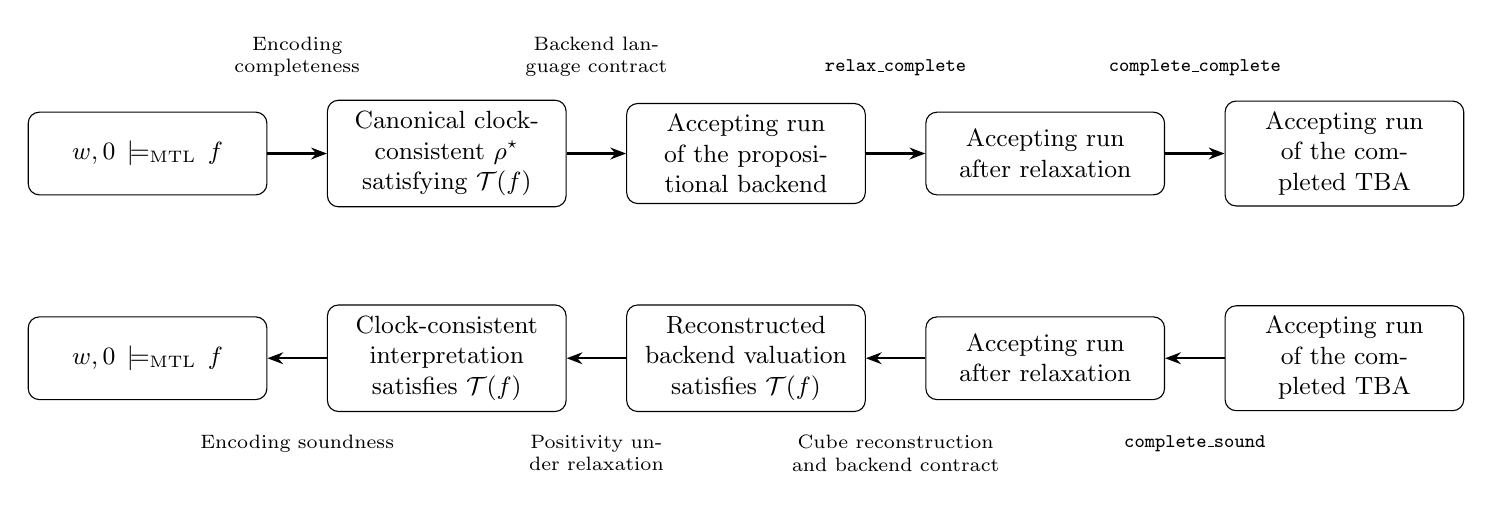
\begin{tikzpicture}[
  proofbox/.style={draw,rounded corners,align=center,text width=2.75cm,
    minimum height=1.05cm,font=\small,inner sep=4pt},
  flow/.style={-{Stealth[length=2mm]},thick},
  flowlabel/.style={font=\scriptsize,align=center,text width=2.65cm,fill=white}
]
\node[proofbox] (mtl) at (0,0) {$w,0\satM f$};
\node[proofbox] (enc) at (3.8,0) {Canonical clock-consistent
  $\rho^\star$ satisfying $\T(f)$};
\node[proofbox] (pb) at (7.6,0) {Accepting run of the
  propositional backend};
\node[proofbox] (relax) at (11.4,0) {Accepting run after
  relaxation};
\node[proofbox] (tba) at (15.2,0) {Accepting run of the
  completed TBA};
\draw[flow] (mtl.east) -- node[flowlabel,above=0.85cm] {Encoding
  completeness} (enc.west);
\draw[flow] (enc.east) -- node[flowlabel,above=0.85cm] {Backend language
  contract} (pb.west);
\draw[flow] (pb.east) -- node[flowlabel,above=0.85cm] {\texttt{relax\_complete}}
  (relax.west);
\draw[flow] (relax.east) -- node[flowlabel,above=0.85cm]
  {\texttt{complete\_complete}} (tba.west);

\node[proofbox] (mtls) at (0,-2.6) {$w,0\satM f$};
\node[proofbox] (encs) at (3.8,-2.6) {Clock-consistent
  interpretation satisfies $\T(f)$};
\node[proofbox] (pbs) at (7.6,-2.6) {Reconstructed backend
  valuation satisfies $\T(f)$};
\node[proofbox] (relaxs) at (11.4,-2.6) {Accepting run after
  relaxation};
\node[proofbox] (tbas) at (15.2,-2.6) {Accepting run of the
  completed TBA};
\draw[flow] (tbas.west) -- node[flowlabel,below=0.85cm]
  {\texttt{complete\_sound}} (relaxs.east);
\draw[flow] (relaxs.west) -- node[flowlabel,below=0.85cm]
  {Cube reconstruction and backend contract} (pbs.east);
\draw[flow] (pbs.west) -- node[flowlabel,below=0.85cm]
  {Positivity under relaxation} (encs.east);
\draw[flow] (encs.west) -- node[flowlabel,below=0.85cm]
  {Encoding soundness} (mtls.east);
\end{tikzpicture}}%
\caption{Proof outline for Theorem~\ref{thm:mtl-to-tba-correct}:
completeness (top) and soundness (bottom), each using the backend equivalence
contract.}
\label{fig:correctness-composition}
\end{figure*}

The convenience theorem \Rocqid{MTL_to_TBA_correct} chooses its backend
using the project axiom \Rocqid{LTL_TO_BUCHI_CORRECT}. It is not
assumption-free. The theorem displayed above instead takes backend
equivalence as an explicit argument. This distinction is visible in
\texttt{proof/ASSUMPTIONS.txt}.

\subsection{Rocq result map}
\label{subsec:rocq-result-map}
Table~\ref{tab:rocq-result-map} maps the article's results to their checked
declarations and assumptions. The primitive rows collect the four soundness
and four canonical-completeness families, each with its strict variant.
\begin{table*}[t]
\centering
\caption{Map from the article's results to Rocq declarations, source modules
(Core, Proof; file names below) and assumptions.}
\label{tab:rocq-result-map}
\begin{tabular}{@{}p{0.18\textwidth}p{0.32\textwidth}p{0.10\textwidth}p{0.26\textwidth}@{}}
\toprule
Mathematical result & Rocq declaration(s) & Source module & Key dependency\\
\midrule
Derived ordinary-operator semantics &
Eight strict/non-strict compatibility lemmas &
Core &
Well-formed real bounds and strictly increasing timed words\\
Canonical correctness at each path; one extension &
\Rocqid{canonical_encoding_all};
\Rocqid{EncodingCorrect_proved} &
Proof &
Standard Rocq real/classical and function-extensionality assumptions\\
Primitive soundness and canonical completeness &
\Rocqid{sound_UhatLe/Ge/Lt/Gt},
\Rocqid{sound_RhatLe/Ge/Lt/Gt};
corresponding \Rocqid{complete_*} lemmas &
Proof &
Soundness: any consistent resets; completeness: canonical policy\\
Relaxation and reset completion &
\Rocqid{relax_sound}, \Rocqid{relax_complete},
\Rocqid{complete_sound}, \Rocqid{complete_complete} &
Core &
Positive extended atoms; label side conditions\\
Conditional backend composition &
\Rocqid{MTL_to_TBA_correct_with} &
Proof &
Explicit backend equivalence premise on action-consistent propositional words\\
Convenience backend theorem &
\Rocqid{MTL_to_TBA_correct} &
Proof &
Project axiom plus standard Rocq assumptions\\
\bottomrule
\end{tabular}
\end{table*}

The source-module aliases in Table~\ref{tab:rocq-result-map} are:
\begin{description}
\item[Core.] \texttt{MTL\_to\_TBA\_Shared\_}\\
\texttt{Clock\_Derived\_Strict\_Direct\_Core.v}
\item[Proof.] \texttt{EncodingCorrect\_Shared\_}\\
\texttt{Clock\_Derived\_Strict\_Direct\_Proof.v}

\end{description}

The assumptions report (the \texttt{Print Assumptions} output of Rocq for each
main theorem, saved as \path{proof/ASSUMPTIONS.txt}) lists standard library
dependencies for classical real comparison
decisions, excluded middle, functional extensionality, and descriptions.
These are distinct from the project-specific backend axiom. The theorem
\Rocqid{MTL_to_TBA_correct_with} has no
\Rocqid{LTL_TO_BUCHI_CORRECT} dependency; its backend premise
is explicit. The convenience theorem does use that axiom. 

The formal domain remains deliberately bounded: well-formed core formulas;
real-valued mathematical parameters (not executable encodings of arbitrary
reals); strictly increasing divergent timestamps; event-guarded automata
without location invariants. Parsing, a concrete LTL backend implementation, Spot execution, graph import, and
automaton printing remain outside
the theorem. The sizes and checks of
Section~\ref{sec:evaluation} are measurements, not mechanized results.

The occurrence-indexed induction, residual invariants, and separate
relaxation/reset-completion obligations expose the proof dependencies behind
the language-preservation result. The development is supplied as inspectable
Rocq source; the successful source replay procedure is
documented with the artifact.
\subsection{Alarm-response proof instance}
\label{sec:alarm-example}
Consider $f_{\mathit{alarm}}=\mathsf{G}(\mathit{alarm}\Rightarrow
\Diamond_{\le 3}\mathit{handled})$, meaning every alarm must be handled within
three time units. In
\Rocqid{proof/OverlappingResponse_Example.v}, the formula is
\texttt{MR MFalse (MOr (MNotAtom ALARM) (MUle 3 MTrue (MAtom HANDLED)))},
where \texttt{ALARM} and \texttt{HANDLED} are actions 1 and 2. Rocq checks
that it is well formed and has one primitive timed subformula,
$\widehat{\mathsf{U}}_{\le 3}\,\top\,\mathit{handled}$, whose obligations
share clock $x$. The translation contains the negated event atom
$\mathsf{LNAct}(\mathit{alarm})$, which the tool prints as the explicit
negation $\neg\mathit{alarm}$ of the event atom. Spot therefore
receives
\begin{multline*}
\mathsf{G}\bigl(\neg\mathit{alarm}\lor \mathit{handled}\lor
\Next((x\le3\land\Unch(x))\\
\qquad\Until(x\le3\land\mathit{handled}))\bigr).
\end{multline*}
Spot 2.16's input and output are saved in
\Rocqid{examples/spot/alarm_response_backend.ltl} and
\Rocqid{examples/spot/alarm_response_backend.dot}~\cite{[spot]}. The generated
automaton, Fig.~\ref{fig:alarm-backend}, has initial state 0 and accepting
states $\{0,1\}$.
\begin{figure*}[t]
\centering
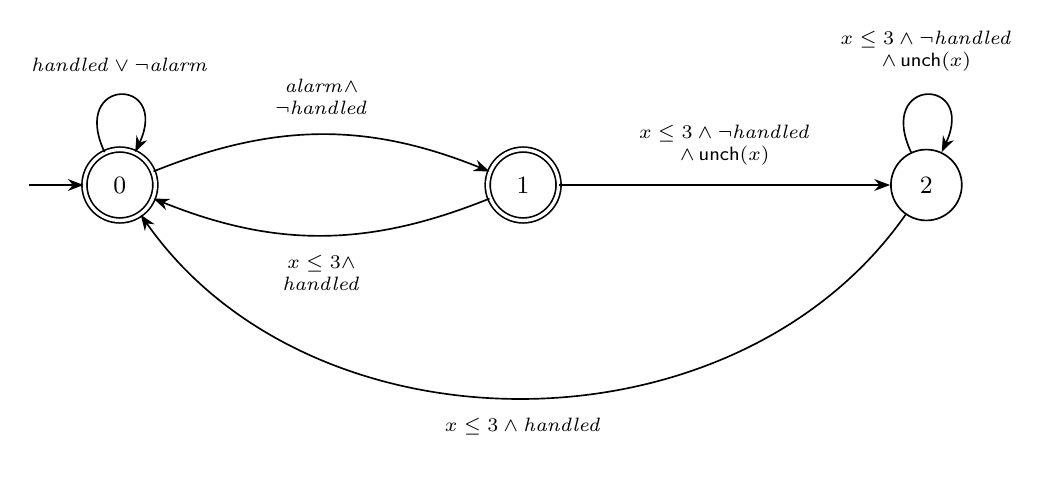
\begin{tikzpicture}[node distance=42mm]
  \node[fmaccept] (q0) {$0$};
  \node[fmaccept,right=of q0] (q1) {$1$};
  \node[fmstate,right=of q1] (q2) {$2$};
  \draw[fmedge] ([xshift=-7mm]q0.west) -- (q0.west);
  \draw[fmedge] (q0) edge[out=115,in=65,looseness=7] node[fmlabel,above=2.5mm]
    {$\mathit{handled}\lor\neg\mathit{alarm}$} (q0);
  \draw[fmedge] (q0) edge[bend left=22] node[fmlabel,above=2mm]
    {$\mathit{alarm}\land$\\$\neg\mathit{handled}$} (q1);
  \draw[fmedge] (q1) edge[bend left=22] node[fmlabel,below=2mm]
    {$x\le3\land$\\$\mathit{handled}$} (q0);
  \draw[fmedge] (q1) -- node[fmlabel,above=2mm]
    {$x\le3\land\neg\mathit{handled}$\\$\land\,\Unch(x)$} (q2);
  \draw[fmedge] (q2) edge[out=115,in=65,looseness=7] node[fmlabel,above=2.5mm]
    {$x\le3\land\neg\mathit{handled}$\\$\land\,\Unch(x)$} (q2);
  \draw[fmedge] (q2) edge[bend left=55] node[fmlabel,below=2mm]
    {$x\le3\land\mathit{handled}$} (q0);
\end{tikzpicture}
\caption{Propositional B\"uchi automaton generated by Spot for the
alarm-response formula. Edges are labeled by the full Boolean condition on
event and clock atoms. Double circles are accepting states, the incoming arrow
marks the initial state, $\Unch(x)$ is the preservation marker, and state
numbers are Spot's.}
\label{fig:alarm-backend}
\end{figure*}
Rocq splits the disjunctive self-loop into two cubes. Lemma
\Rocqid{alarm_response_T_eq} matches its input to the Rocq translation;
\Rocqid{alarm_response_spot_backend_contract} proves that the transcribed
automaton has exactly that LTL language on the action-consistent propositional
words, which is the contract above. 
The resulting concrete TBA is \Rocqid{alarm_response_spot_tba}. It has initial
location $0$, accepting locations $\{0,1\}$, and clock $x$.
Figure~\ref{fig:alarm-tba} shows the reset-completed automaton of the Rocq
record. Each edge is labeled by its event, its clock guard, and its resets;
guards are checked before resets, and an edge without a guard has none. The
two edges from $0$ to $0$ of the record are drawn as one edge with two labels.
\begin{figure*}[t]
\centering
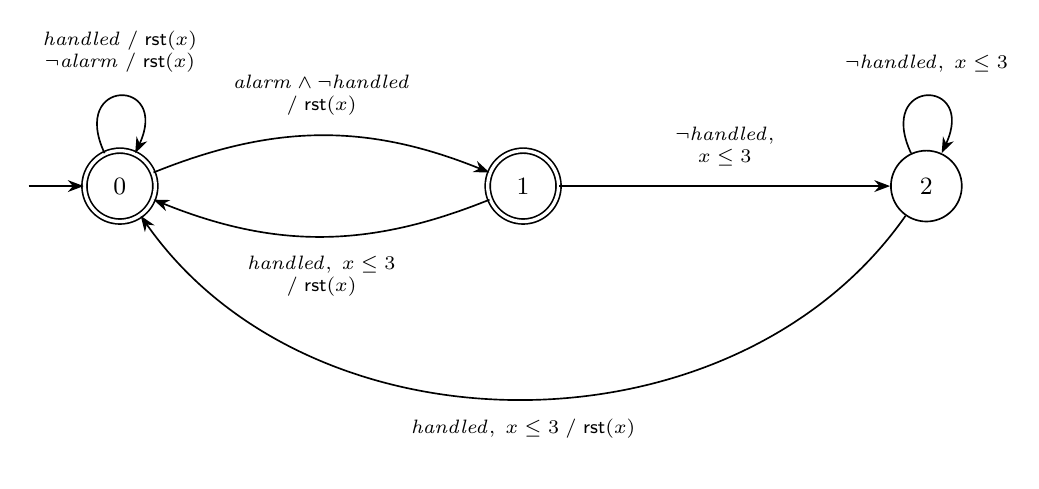
\begin{tikzpicture}[node distance=42mm]
  \node[fmaccept] (q0) {$0$};
  \node[fmaccept,right=of q0] (q1) {$1$};
  \node[fmstate,right=of q1] (q2) {$2$};
  \draw[fmedge] ([xshift=-7mm]q0.west) -- (q0.west);
  \draw[fmedge] (q0) edge[out=115,in=65,looseness=7] node[fmlabel,above=2.5mm]
    {$\mathit{handled}\;/\;\mathsf{rst}(x)$\\$\neg\mathit{alarm}\;/\;\mathsf{rst}(x)$} (q0);
  \draw[fmedge] (q0) edge[bend left=22] node[fmlabel,above=2mm]
    {$\mathit{alarm}\land\neg\mathit{handled}$\\$/\;\mathsf{rst}(x)$} (q1);
  \draw[fmedge] (q1) edge[bend left=22] node[fmlabel,below=2mm]
    {$\mathit{handled},\;x\le3$\\$/\;\mathsf{rst}(x)$} (q0);
  \draw[fmedge] (q1) -- node[fmlabel,above=2mm]
    {$\neg\mathit{handled},$\\$x\le3$} (q2);
  \draw[fmedge] (q2) edge[out=115,in=65,looseness=7] node[fmlabel,above=2.5mm]
    {$\neg\mathit{handled},\;x\le3$} (q2);
  \draw[fmedge] (q2) edge[bend left=55] node[fmlabel,below=2mm]
    {$\mathit{handled},\;x\le3\;/\;\mathsf{rst}(x)$} (q0);
\end{tikzpicture}
\caption{Timed automaton of the alarm-response Rocq record after relaxation
and reset completion. Edges are labeled by event, clock guard and, after a
slash, the clocks reset; double circles are accepting states. The Graphviz DOT
graph-to-record correspondence remains outside the Rocq proof.}
\label{fig:alarm-tba}
\end{figure*}
The theorem \Rocqid{alarm_response_spot_tba_correct} instantiates
Theorem~\ref{thm:mtl-to-tba-correct} and proves that this record accepts
exactly the timed words satisfying $f_{\mathit{alarm}}$.


\section{Evaluation}
\label{sec:evaluation}
The theorem says nothing about the size of the automaton, about the
unverified components that produce it, or about how it compares with an
independent implementation. This section measures the automaton
$\mathsf{compile}(f)$ obtained by the translation $\T$, Spot, relaxation, and
reset completion, before any further processing; no optimization or export
is applied here. We ask three questions. Q1: how large is
$\mathsf{compile}(f)$, compared with the automaton of CASAAL~\cite{casaal_tool},
which implements the construction of Li et al.~\cite{li_spin7}? Q2: on
concrete formulas, do the languages agree with CASAAL's, as far as an
independent timed-automaton checker, or independent evaluation on words, can
tell? Q3: does the backend satisfy,
on these formulas, the contract that the theorem assumes? The answers are
measurements and tests; none of them is a mechanized result.

\subsection{Setup}
The tool \texttt{mtl2tba} parses a formula, computes $\T(f)$, calls Spot~2.16
(\texttt{ltl2tgba}), reads its LBTT output, and applies relaxation and reset
completion. The functions $\T$, relaxation, and reset completion are OCaml
code extracted from the Rocq definitions; the parser, the call to Spot, the
LBTT reader, the printers, and extraction itself are not verified. The tool is
run with the options \texttt{-noweak -norecur}, so that the clocked-LTL
formula is exactly $\T(f)$ as defined in Section~\ref{sec:translation}.
Measurements were taken on an Intel Core i7-8650U (1.9~GHz, 11.7~GB) under
Ubuntu~26.04 in WSL~2, with a limit of 600~s per tool run and per check
(120~s for random formulas). The 31 configurations are fifteen
specification patterns F1--F14 (F3b is F3 without hat), conjunctions R$k$ of
$k$ bounded responses $\Box(a_i\Rightarrow\Diamond_{\le5}b_i)$ for
$k=1,\dots,8$, and nestings N$k$ of $k$ bounded eventualities
$\Diamond_{\le5}(p_1\land\Diamond_{\le5}(p_2\land\cdots))$. Scripts, inputs,
CASAAL outputs, and raw results are in the artifact
(\path{evaluation/}).

\subsection{Size of compile(f) and CASAAL reference}
Table~\ref{tab:compiled} gives, for each configuration, the reachable
locations, transitions, and clocks of $\mathsf{compile}(f)$, and the size of
CASAAL's output. CASAAL was run with mutually exclusive events, which matches
our one-event-per-position words. The two counts of transitions are not
directly comparable: CASAAL labels a transition with a Boolean formula over
propositions, whereas Spot's output, and hence $\mathsf{compile}(f)$, has one
transition per cube over the propositions and clock literals. In R4, for
example, $\mathsf{compile}(f)$ has 48 locations and 1,625 transitions, and
CASAAL 16 locations and 80 symbolic transitions; both use four clocks.
Column Grp.~T counts the transitions of $\mathsf{compile}(f)$ after grouping
edges with the same source, target, guard, and resets into one edge labelled by
the union of their events; it is a way of counting and changes no automaton.
Grouping reduces R4 from 1,625 to 768 and N8 from 166 to 54 transitions, but a
gap remains (CASAAL: 80 and 19), so the difference is not explained by the
representation of labels alone.
\begin{table}[t]
\centering
\caption{Automaton $\mathsf{compile}(f)$ before any optimization: locations/transitions/clocks (L/T/X), the transitions after grouping edges with the same source, target, guard, and resets into one (Grp.\ T; a count, not a transformation), CASAAL output with mutually exclusive events (locations/symbolic transitions/clocks; n/a: no exact CASAAL encoding), TChecker products $P_1,P_2,S$ (``empty'': all three empty), and the tested backend contract.}
\label{tab:compiled}
\scriptsize
\setlength{\tabcolsep}{3pt}
\begin{tabular}{@{}lrrrcc@{}}
\toprule
ID & L/T/X & Grp.\ T & CASAAL & $P_1,P_2,S$ & Backend\\
\midrule
F1 & 3/7/1 & 6 & 2/4/1 & empty & yes\\
F2 & 2/5/1 & 5 & 1/1/0 & empty & yes\\
F3 & 2/5/1 & 5 & n/a & S only & yes\\
F3b & 1/1/0 & 1 & 1/1/0 & empty & yes\\
F4 & 3/7/1 & 6 & 2/4/1 & empty & yes\\
F5 & 7/38/1 & 34 & 4/15/1 & empty & yes\\
F6 & 7/38/1 & 34 & 4/15/1 & empty & yes\\
F7 & 3/6/1 & 6 & 2/4/1 & empty & yes\\
F8 & 5/15/1 & 15 & 2/4/1 & empty & yes\\
F9 & 4/9/2 & 9 & 4/9/2 & empty & yes\\
F10 & 5/13/3 & 12 & 5/12/3 & empty & yes\\
F11 & 5/11/2 & 11 & 4/7/2 & empty & yes\\
F12 & 5/23/2 & 23 & 3/9/2 & empty & yes\\
F13 & 6/23/2 & 23 & n/a & S only & yes\\
F14 & 8/38/2 & 29 & 8/18/2 & empty & yes\\
R1 & 3/7/1 & 6 & 2/4/1 & empty & yes\\
R2 & 8/45/2 & 32 & 4/12/2 & empty & yes\\
R3 & 20/275/3 & 160 & 8/32/3 & empty & yes\\
R4 & 48/1625/4 & 768 & 16/80/4 & timeout & yes\\
R5 & 112/9375/5 & 3584 & 32/192/5 & timeout & yes\\
R6 & timeout & -- & 64/448/6 & -- & yes\\
R7 & timeout & -- & 128/1024/7 & -- & check timeout\\
R8 & timeout & -- & 256/2304/8 & -- & tool timeout\\
N1 & 3/5/1 & 5 & 3/5/1 & empty & yes\\
N2 & 4/11/2 & 9 & 4/7/2 & empty & yes\\
N3 & 5/21/3 & 14 & 5/9/3 & empty & yes\\
N4 & 6/36/4 & 20 & 6/11/4 & empty & yes\\
N5 & 7/57/5 & 27 & 7/13/5 & timeout & yes\\
N6 & 8/85/6 & 35 & 8/15/6 & timeout & yes\\
N7 & 9/121/7 & 44 & 9/17/7 & timeout & yes\\
N8 & 10/166/8 & 54 & 10/19/8 & timeout & ltl2ba timeout\\
\bottomrule
\end{tabular}
\end{table}


The number of clocks coincides with CASAAL's on every configuration that
CASAAL encodes exactly, except F2: under mutual exclusion,
$\Box(p\Rightarrow\Box_{\le3}q)$ forbids $p$ altogether, and CASAAL produces a
one-state automaton without clock, whereas $\mathsf{compile}(f)$ keeps two
locations and one clock. This agrees with the clock discipline of the
construction: one clock per structurally distinct primitive timed
subformula. Locations and transitions are larger than CASAAL's on most
configurations, sometimes by a large factor (R4, R5); the nesting family N
has the same number of locations as CASAAL. The growth in the R family comes
from Spot's automaton for the conjunction of $k$ clocked-LTL clauses, before
relaxation; R6--R8 exceed the 600-second limit. Construction time is below
one second for every completed configuration except R4 (3.4~s), N6
(1.6~s), and R5 (43~s). These numbers describe
the unoptimized output of the verified construction; they are not a
comparison of tools; reducing these sizes by post-processing is left to
follow-up work.

\subsection{Language checks with TChecker}
For a formula $\varphi$, let $O$ and $O'$ be $\mathsf{compile}(\varphi)$ and
$\mathsf{compile}(\neg\varphi)$, and $C$, $C'$ CASAAL's automata for
$\varphi$ and $\neg\varphi$. TChecker~0.8~\cite{tchecker} decides the
emptiness of the products $P_1=O\times C'$, $P_2=C\times O'$, and
$S=O\times O'$, built over infinite words with one event per position,
strictly increasing and divergent timestamps, and clocks starting at~0.
$P_1$ and $P_2$ empty mean that $O$ is disjoint from $C'$ and $C$ from $O'$;
if CASAAL's two automata are complementary, which is not checked, this gives
$L(C)\subseteq L(O)$ and $L(C')\subseteq L(O')$. The checks therefore
establish inclusions, not equality. $S$ empty means that our automata for
$\varphi$ and $\neg\varphi$ never accept the same word. A fourth product
$O\times C$ is a sanity check: it must be non-empty when $\varphi$ is
satisfiable.

On the benchmark configurations, $P_1$, $P_2$, and $S$ are empty for every
configuration that completes within the limits (F1--F14 except the hatted F3
and F13, which CASAAL cannot express, R1--R3, and N1--N4); for F3 and F13
only $S$ is checked, and it is empty. For R5 and N6 the three checks exceed 600~s. At 1{,}800~s, run singly, $P_2$ of R4
is empty, while $P_1$, $S$ of R4 and all three checks of N5 still time out (which
may also mean memory exhaustion). R6--R8 produce no automaton within the limit.
For N7 and N8, $O$ is built (26~s and 101~s), but $P_1$ exceeds 600~s and $O'$ is
not built within the limit, so $P_2$ and $S$ are not run (inconclusive).
The sanity product is non-empty in every completed case.

The artifact also contains 100 random formulas of depth at most three over
three propositions, generated with their CASAAL automata. For 99 of them,
$P_1$, $P_2$, and $S$ are empty, with no timeout; for five of these, the
sanity product is empty as well, and inspection shows that each of these
five formulas is unsatisfiable under mutual exclusion (for example
$q\land\Diamond_{>2}p\land r$). The remaining formula, X74, is $\Diamond(q\land r)\Rightarrow
eg p$, for which
$P_1$ is non-empty. Its negation $\Diamond(q\land r)\land p$ is unsatisfiable
under mutual exclusion, and our automaton for it has no accepting location.
CASAAL's printed automaton for the negation has no acceptance mark, and the
conversion script reads an automaton without marks as accepting every run (as for $\mathsf F q\land\mathsf G\neg q$). We report X74 as
inconclusive: it reflects how acceptance is printed and read, not a
disagreement that the products can establish.

\subsection{Agreement on ultimately periodic words}
The TChecker checks establish inclusions and time out on the larger
configurations, so we add a test of equality on finitely many words. For each
configuration we draw random ultimately periodic timed words $uv^\omega$ (a
prefix of 0--4 and a loop of 1--5 events, integer timestamps in half units,
strictly increasing and divergent; half of the words follow the order of the
propositions of the formula), and compare three verdicts: the formula under the
pointwise semantics above, evaluated by an independent Python implementation;
acceptance by $\mathsf{compile}(f)$; and acceptance by CASAAL's automaton.
Clocks of CASAAL start at 0; for $\mathsf{compile}(f)$ initial clock values
are tried on a grid when it has at most three clocks, since the theorem
quantifies them existentially. On the 28 benchmark configurations that build
(400 words each, 11{,}200 in all, 4{,}495 satisfying the formula) and on the
100 random formulas (150 words each, 15{,}000 in all, 8{,}273 satisfying
it), the semantics and $\mathsf{compile}(f)$ agree on every word. CASAAL is included on 26 of the
28 benchmark configurations (not on the hatted F3 and F13) and on all random
formulas, and agrees on every word there as well: 10{,}400 plus 15{,}000
words, 25{,}400 three-way comparisons; the other 800 words compare only the
semantics and the automaton. As a negative control, the same checker finds disagreements for F1
against the formulas with bound 4 instead of 5 (11 of 300 words) and with a
strict bound (5 of 300). The test has little weight for some formulas:
no word of N8 satisfies the formula among the random ones, so for N5--N8 we
added five hand-built words each (accepted and rejected; all agree), and nine
random formulas have fewer than five satisfying and fourteen fewer than five
violating words. The words are finitely many and short; this is a test, not a
proof of equality.

\subsection{Backend contract}
Theorem \Rocqid{MTL_to_TBA_correct_with} assumes that the propositional
automaton accepts exactly the models of $\T(f)$. For each configuration we
saved the formula given to Spot and the LBTT automaton $A$ it returned, and
checked the contract with Spot's \texttt{autfilt}, using an independent
translator, ltl2ba~1.3: $A\times\mathrm{ltl2ba}(\neg\T(f))$ and
$\overline{A}\times\mathrm{ltl2ba}(\T(f))$ must both be empty. The contract
holds on 28 of the 31 configurations; for R7 the check exceeds 600~s, for N8
ltl2ba exceeds 300~s, and for R8 Spot does not finish. On every configuration
where Spot produced an automaton, the number of states and transitions read by
the LBTT reader of \texttt{mtl2tba} equals the number reported by
\texttt{autfilt} on the same file. These checks test the contract on these
inputs; they do not prove it, and they use Spot's own tools for part of the
check.

\subsection{Hatted operators}
F3 and F13 use the hatted operators of Section~\ref{sec:logic}. CASAAL has no
hatted operator; its closest encoding of F3,
$\Box(e\Rightarrow\Next\Box_{\le2}\neg e)$, measures the window from the next
event rather than from the triggering one
(Fig.~\ref{fig:hat-reference}) and is not equivalent, so we do not compare
the two languages. The time reference is visible in the automata. Under mutual exclusion the
non-strict window of the unhatted F3b contains the triggering event, so F3b
forbids $e$ altogether: $\mathsf{compile}(f)$ has one location, one
transition, and no clock. The window of F3 starts after the triggering event
but is measured from its timestamp, and $\mathsf{compile}(f)$ has two
locations, five transitions, and one clock $x$, reset on each $e$; after
an $e$, a further $e$ is accepted only with the guard $x>2$.

\subsection{Threats to validity}
The configurations and random formulas are small and of our choosing; the
R family shows that the size of Spot's automaton grows quickly with the
number of conjuncts. The CASAAL automata were produced earlier and not
regenerated; CASAAL's integer bounds, nondecreasing time, and acceptance
printing differ from our model, and the inclusions depend on the unchecked
complementarity of its automata. The TChecker products, the word-level test,
and the conversion scripts are unverified code. Timeouts are reported as
inconclusive.


\section{Artifact and Reproducibility}
\label{sec:artifact}
The artifact is available at
\url{https://github.com/efares1/rocq-mtl-to-tba-translation};
the revision described here is the release tagged \texttt{v1.2}.
It contains the Rocq sources, the assumptions report, the tool
\texttt{mtl2tba}, the evaluation scripts with their inputs and raw results,
the Spot input and graph of the alarm-response example, and the article
source. The proofs build with Rocq~9.0.1: \texttt{make} in \path{proof/}
compiles the core, the correctness development, and the alarm example;
\path{proof/CheckAssumptions.v} prints the assumptions of the main theorems,
which are recorded in \path{proof/ASSUMPTIONS.txt}; and \texttt{coqchk}
re-checks the compiled objects. On Windows, \path{reproduce-ieee-access.ps1}
performs these steps, runs the two Python assurance scripts, and builds the
PDF. The scripts are executable audits, not verified components:
\path{examples/assurance/check_spot_transcription.py} compares the
Spot graph with the Rocq record of the alarm-response instance, up to state
renaming, including edge guards (with mutation self-tests), and
\path{examples/assurance/reset_policy_scenarios.py} checks the finite
reset-policy scenarios of Table~\ref{tab:overlap-example}.

The main checked claims have direct source declarations:
\Rocqid{EncodingCorrect_proved} and
\Rocqid{canonical_encoding_all} establish the formula-to-clocked-LTL
equivalence; \Rocqid{MTL_to_TBA_correct_with} composes this result with
the explicit backend contract on action-consistent propositional words;
\Rocqid{alarm_response_spot_tba_correct} is the concrete alarm
instance. The primitive theorem families, relaxation lemmas, reset-completion
lemmas, and their assumptions are mapped in
Table~\ref{tab:rocq-result-map}.

The evaluation of Section~\ref{sec:evaluation} is reproduced, under Linux or
WSL with OCaml, Spot~2.16, TChecker~0.8, and ltl2ba~1.3, by building the tool
in \path{tool/} and running \path{evaluation/run_compiled_eval.sh} and
\path{evaluation/run_spot_validation.sh}; \path{evaluation/make_compiled_table.py}
regenerates Table~\ref{tab:compiled} from the raw results. The word-level
test is \path{evaluation/lasso_check.py}, run on the automata written by
\path{evaluation/dump_compile_dot.sh}, and \path{evaluation/grouped_edges.py}
computes the grouped transition counts.

\section{Related Work}
\label{sec:related}
\begin{table*}[!t]
\centering
\caption{Representative mathematical results and mechanization evidence for
timed-logic-to-automata constructions. The rows have different logics,
semantics, targets, and proof scopes; they are not a performance comparison.}
\label{tab:prior-construction-comparison}
\begin{tabular}{@{}p{0.12\textwidth}p{0.20\textwidth}p{0.34\textwidth}p{0.23\textwidth}@{}}
\toprule
Work & Semantic scope & Existing correctness and construction & Mechanization and implementation evidence\\
\midrule
Bulychev~\cite{[BDLG14]} & Pointwise non-Zeno infinite words; integer bounds, all four comparisons, nondecreasing timestamps. & Theorems 1--2 prove exact automaton languages for safety/co-safety. The construction extends the classical tableau LTL-to-B\"uchi translation directly, with timed-subformula clocks, obligations, and reset/unchanged markers. & Mathematical proofs and controller-synthesis tooling for the stated fragments.\\
Li et al.~\cite{li_spin7} & Full MTL$_{0,\infty}$; pointwise non-Zeno words, integer bounds, all four comparisons, nondecreasing timestamps, zero initial clocks. & Establishes exact language equality for the timed-B\"uchi construction (closure, extended formulas, degeneralization) and language preservation under best-choice resets. & CASAAL implements the workflow and deterministic approximations~\cite{casaal_tool}; the proof is mathematical.\\
Xu and Miao~\cite{xu08} & MITL formulas mapped to fair timed automata; exact semantic relation to this paper's pointwise event-word model is not compared. & One tester automaton per subformula, with local clocks measuring elapsed time against the metric interval, composed in parallel; no intermediate untimed LTL stage. & The construction and its implementation in PVS.\\
This paper & Well-formed Rocq formulas with real bounds, strictly increasing timestamps, existential nonnegative initial clocks. & Translation factored through clocked LTL and a standard LTL-to-B\"uchi backend. \Rocqid{EncodingCorrect_proved} proves clocked-LTL equivalence for all eight primitive cases; TBA composition is conditional on backend equivalence. & Rocq-checked proof and one proved contract for a manual Spot transcription; tool evaluation with extracted code (Section~\ref{sec:evaluation}).\\
\bottomrule
\end{tabular}
\end{table*}

Pointwise MTL has extensive decidability and expressiveness results
\cite{[RK90],[RTH96],MTLsem,ouaknine_worrell_lics05,
bouyer_chevalier_markey_fsttcs05}. Unrestricted dense-time MTL has no general
effective translation to finite ordinary timed automata; bounded-variability
and alternating-automaton results have different scopes
\cite{nickovic_piterman_formats10,[BM14]}. MTL$_{0,\infty}$ retains common
response and separation properties~\cite{[RTH96],[BDLG14]}. Our hatted
operators make the timing reference explicit in the logic and proof.

\runinhead{Translations of timed logics.}
Li et al. establish the full-fragment mathematical language-equivalence
result. Our overlapping-activation proof checks completeness for the present
formal model; we do not infer that prior constructions lacked such handling.

Bulychev et al. state that their translation uses ``the classical
tableau-based translation from linear-time temporal formulas into B\"uchi
automata'' with two modifications: no B\"uchi acceptance condition for the
safety and co-safety fragments, and an auxiliary clock for each timed
subformula. Li et al. proceed by a closure, extended formulas that carry the
clock bookkeeping, a normal form, a transition-based timed B\"uchi automaton,
and a degeneralization step. In both, as we read them, the timed expansion and the B\"uchi
construction are one hand-built construction. Ours differs in architecture:
the formula is encoded into untimed clocked LTL, any LTL-to-B\"uchi backend
may then be used, and its correctness enters the composed theorem as an
explicit contract. This factoring is what the Rocq development exploits, and
it is also why the backend premise is separate from the timed argument.
To the best of our knowledge, none of the translations from MTL or MITL to
timed automata that we examined (the two above, the testers of Maler et al.,
MightyL, MightyPPL, and Xu and Miao) is presented in this form; we did not examine every
cited work in the same depth.

Xu and Miao describe a PVS-based transformation from MITL formulas to fair
timed automata, including construction principles and implementation
details~\cite{xu08}. Their construction builds one tester automaton per
subformula, each with local clocks that measure the elapsed time against the
metric interval, and composes the testers in parallel; it has no intermediate
untimed LTL stage. This is an earlier proof-assistant-based timed-logic
translation; our scope-specific comparison concerns the pointwise
MTL$_{0,\infty}$ construction formalized here.

MITL translations use temporal testers, automata networks, or one-clock
alternating automata~\cite{maler_mitl_to_ta,
ferrere2019_realtimelogic_to_ta,[BM14]}; MightyL and MITL2Timed provide
UPPAAL-oriented tools for that distinct logic
\cite{mightyl_paper17,mitl2timed_github}. MightyL, for example, outputs a
network of timed automata, one per temporal subformula, generalizing the
Gastin--Oddoux LTL-to-B\"uchi construction; as described in~\cite{mightyl_paper17}, it does not call an LTL-to-B\"uchi
tool on a timed formula. Obligation-merging techniques are
related, while our one-sided residual predicates support the checked
completeness proof.

\runinhead{Clocked temporal logic and subformula clocks.}
The clocked linear temporal logic extension CLTLoc adds clock comparisons and reset predicates and has been used to
encode metric logics~\cite{bersani_cltloc}. Our similar propositional
vocabulary is an automaton-synthesis intermediate: the backend treats clock
tests and reset markers as propositions. Positivity gives upward closure, and
reset completion restores timed meaning; hence the explicit relaxation proof.

Event-clock logics associate clocks with subformulas to measure time since or
until events~\cite{afh_eventclock_tcs99,
raskin_schobbens_jalc99,nickovic_piterman_formats10}. Formula-indexed clocks
are established; our proof checks that one clock per distinct timed formula
preserves language across repeated activations and all
cases (Section~\ref{subsec:occurrence-induction}).

\runinhead{Recent automata-based real-time verification.}
Recent neighboring work addresses different settings: an improved one-clock
alternating MTL automaton for finite timed words with clock deactivation and
zone analysis~\cite{bouyer_srivathsan_vishwanath_fossacs25}; and TEMPORA's
pointwise MITL model checking with past and future modalities
~\cite{akshay_et_al_tempora26}. These do not
translate our MTL$_{0,\infty}$ fragment to infinite-word TBAs.
Ho et al.'s MightyPPL translates pointwise MITL with past and Pnueli
modalities over finite and infinite timed words; it gives mathematical
construction results and proof sketches alongside a complete implementation
whose testers sequentialize overlapping obligations~\cite{mightyppl_tacas26}. A companion
preprint~\cite{mightyppl_qest_arxiv26} describes
an implementation for existentially punctual metric temporal logic with past
and Pnueli modalities (MTLPPL). Its term
\emph{one-sided MTL} denotes the subfragment without past or Pnueli, whereas
here it describes interval shapes $[0,d]$ and $[d,\infty)$. Any syntactic
containment comparison is limited to conventional source formulas after
zero-bound reduction and with integer bounds; it excludes hatted abstract syntax tree (AST)
constructors. The QEST fragment also permits punctual and non-one-sided
intervals in its stated positions. Its punctual-response example does not
imply support for unrestricted punctual MTL; differing bounds and timed-word
conventions preclude a shared-input semantic comparison.

These tools (TEMPORA, MightyPPL, and the alternating-automaton work above)
address different fragments or output models; this paper neither re-verifies
them nor makes a shared-input, coverage, clock-count, or performance
comparison with them. The Rocq development is not integrated with CASAAL,
MightyPPL, or another checker.

\runinhead{Mechanized translations and trusted backends.}
Proof-assistant work already verifies LTL-to-B\"uchi constructions and model
checkers~\cite{schimpf_tphols09,cava_cav13,ltl_to_gba_afp,
seidl_sickert_afp19}. Wang et al. verify an MLTL-to-regular-expression
transformation in Isabelle/HOL, export executable code, and compare it with
existing implementations~\cite{wang_mltl_tacas25}. Chattopadhyay and
Mamouras formalize in Coq a compositional construction of online monitors for
past-time MTL over a discrete temporal domain, using quantitative semantics
and Moore machines; they also extract OCaml monitors. This is a distinct
monitoring target and semantic setting from the infinite-word TBA construction
studied here~\cite{chattopadhyay_mamouras_rv20}. For metric logics, Roohi
and Viswanathan use PVS to correct an unsound release semantics in prior MITL
decision procedures and prove supporting results for an adapted
timed-automata construction under continuous-time signal semantics
~\cite{roohi_viswanathan_vmcai18}. Xu and Miao's PVS-based construction is
described above. Together, these works establish substantial proof-assistant
precedents for related metric logics, monitors, and automata; this paper adds a
Rocq-checked correctness development for the specified pointwise infinite-word
TBA construction.

\runinhead{Event-B refinement patterns.}
The context of this work is the generation of Event-B patterns from timed
formulas: the TBA translation studied here is intended as the input of a later
pattern-generation step. Our earlier work on Event-B patterns covers their
DSL-based generation~\cite{fares_abz23}, their derivation through weakest
preconditions~\cite{fares_facs24}, and predicate transformers~\cite{fares_scp27}.
The present paper covers the MTL-to-TBA stage only and gives no TBA-to-Event-B
transformation.

\section{Conclusion}
This paper provides a Rocq-checked soundness-and-completeness development for
the specified pointwise MTL$_{0,\infty}$-to-TBA construction. Its proof covers
all eight primitive cases, soundness for arbitrary
clock-consistent reset traces, and completeness using one canonical trace
across repeated activations of formula-keyed clocks. The occurrence-indexed
induction connects each syntactic occurrence to its translation while
preserving the identity of a shared clock. This supplies a checked account of
the obligations that a mathematical argument must discharge when several
timed requirements overlap.

Rocq also checks relaxation and reset completion and composes them with an
explicit propositional backend language-equivalence contract. The resulting
theorem makes its backend dependency inspectable instead of hiding it in an
assurance claim. This work builds on the mathematical language-preservation
results of Li et al. and adjacent proof-assistant work, while contributing a
reformulation that factors the
translation through untimed clocked LTL and a standard LTL-to-B\"uchi backend,
and a machine-checked derivation for this
construction and the semantic model defined here~\cite{li_spin7,xu08,roohi_viswanathan_vmcai18}.

The evaluation of the extracted construction found no disagreement with CASAAL
on the checked configurations and words, and no discrepancy of the backend
contract on 28 of the 31 configurations; the larger configurations are
inconclusive.

The theorem applies to the stated pointwise semantics and composes
through an explicit backend contract. The contract is discharged only for a
manually transcribed backend record in the alarm-response instance, and
Spot's graph generation/import and zero-bound preprocessing remain outside
the checked boundary. Future work
can extend the mechanization to these components and connect the semantic
theorem to a verified executable backend.

The proof artifact and assumptions report are described in
Section~\ref{sec:artifact}.

\bibliographystyle{IEEEtran}
\bibliography{references}
\begin{IEEEbiographynophoto}{Elie Fares}
Elie Fares is with the Higher Colleges of Technology, Sharjah, UAE. His
research interests include formal methods, refinement-based development and mechanized verification.
\end{IEEEbiographynophoto}

\begin{IEEEbiographynophoto}{Jean-Paul Bodeveix}
Jean-Paul Bodeveix is with IRIT, Universit\'e de Toulouse, France. His research
interests include formal methods, semantic models, refinement-based correct-by-construction development, and proof assistants.
\end{IEEEbiographynophoto}

\begin{IEEEbiographynophoto}{Hussain Al-Aqrabi}
Hussain Al-Aqrabi is with the Higher Colleges of Technology, Sharjah, UAE. His
research interests include cybersecurity and cloud security.
\end{IEEEbiographynophoto}

\begin{IEEEbiographynophoto}{Azar Salami}
Azar Salami is with the Higher Colleges of Technology, Sharjah, UAE. His research interests
include mathematics and formal methods.\EOD
\end{IEEEbiographynophoto}
\end{document}
